% Options for packages loaded elsewhere
\PassOptionsToPackage{unicode}{hyperref}
\PassOptionsToPackage{hyphens}{url}
%
\documentclass[
]{article}
\usepackage{lmodern}
\usepackage{amssymb,amsmath}
\usepackage{ifxetex,ifluatex}
\ifnum 0\ifxetex 1\fi\ifluatex 1\fi=0 % if pdftex
  \usepackage[T1]{fontenc}
  \usepackage[utf8]{inputenc}
  \usepackage{textcomp} % provide euro and other symbols
\else % if luatex or xetex
  \usepackage{unicode-math}
  \defaultfontfeatures{Scale=MatchLowercase}
  \defaultfontfeatures[\rmfamily]{Ligatures=TeX,Scale=1}
\fi
% Use upquote if available, for straight quotes in verbatim environments
\IfFileExists{upquote.sty}{\usepackage{upquote}}{}
\IfFileExists{microtype.sty}{% use microtype if available
  \usepackage[]{microtype}
  \UseMicrotypeSet[protrusion]{basicmath} % disable protrusion for tt fonts
}{}
\makeatletter
\@ifundefined{KOMAClassName}{% if non-KOMA class
  \IfFileExists{parskip.sty}{%
    \usepackage{parskip}
  }{% else
    \setlength{\parindent}{0pt}
    \setlength{\parskip}{6pt plus 2pt minus 1pt}}
}{% if KOMA class
  \KOMAoptions{parskip=half}}
\makeatother
\usepackage{xcolor}
\IfFileExists{xurl.sty}{\usepackage{xurl}}{} % add URL line breaks if available
\IfFileExists{bookmark.sty}{\usepackage{bookmark}}{\usepackage{hyperref}}
\hypersetup{
  pdftitle={FIT5209 Assignment 1 - Linear Regression},
  pdfauthor={Bethany Hooper},
  hidelinks,
  pdfcreator={LaTeX via pandoc}}
\urlstyle{same} % disable monospaced font for URLs
\usepackage[margin=1in]{geometry}
\usepackage{color}
\usepackage{fancyvrb}
\newcommand{\VerbBar}{|}
\newcommand{\VERB}{\Verb[commandchars=\\\{\}]}
\DefineVerbatimEnvironment{Highlighting}{Verbatim}{commandchars=\\\{\}}
% Add ',fontsize=\small' for more characters per line
\usepackage{framed}
\definecolor{shadecolor}{RGB}{248,248,248}
\newenvironment{Shaded}{\begin{snugshade}}{\end{snugshade}}
\newcommand{\AlertTok}[1]{\textcolor[rgb]{0.94,0.16,0.16}{#1}}
\newcommand{\AnnotationTok}[1]{\textcolor[rgb]{0.56,0.35,0.01}{\textbf{\textit{#1}}}}
\newcommand{\AttributeTok}[1]{\textcolor[rgb]{0.77,0.63,0.00}{#1}}
\newcommand{\BaseNTok}[1]{\textcolor[rgb]{0.00,0.00,0.81}{#1}}
\newcommand{\BuiltInTok}[1]{#1}
\newcommand{\CharTok}[1]{\textcolor[rgb]{0.31,0.60,0.02}{#1}}
\newcommand{\CommentTok}[1]{\textcolor[rgb]{0.56,0.35,0.01}{\textit{#1}}}
\newcommand{\CommentVarTok}[1]{\textcolor[rgb]{0.56,0.35,0.01}{\textbf{\textit{#1}}}}
\newcommand{\ConstantTok}[1]{\textcolor[rgb]{0.00,0.00,0.00}{#1}}
\newcommand{\ControlFlowTok}[1]{\textcolor[rgb]{0.13,0.29,0.53}{\textbf{#1}}}
\newcommand{\DataTypeTok}[1]{\textcolor[rgb]{0.13,0.29,0.53}{#1}}
\newcommand{\DecValTok}[1]{\textcolor[rgb]{0.00,0.00,0.81}{#1}}
\newcommand{\DocumentationTok}[1]{\textcolor[rgb]{0.56,0.35,0.01}{\textbf{\textit{#1}}}}
\newcommand{\ErrorTok}[1]{\textcolor[rgb]{0.64,0.00,0.00}{\textbf{#1}}}
\newcommand{\ExtensionTok}[1]{#1}
\newcommand{\FloatTok}[1]{\textcolor[rgb]{0.00,0.00,0.81}{#1}}
\newcommand{\FunctionTok}[1]{\textcolor[rgb]{0.00,0.00,0.00}{#1}}
\newcommand{\ImportTok}[1]{#1}
\newcommand{\InformationTok}[1]{\textcolor[rgb]{0.56,0.35,0.01}{\textbf{\textit{#1}}}}
\newcommand{\KeywordTok}[1]{\textcolor[rgb]{0.13,0.29,0.53}{\textbf{#1}}}
\newcommand{\NormalTok}[1]{#1}
\newcommand{\OperatorTok}[1]{\textcolor[rgb]{0.81,0.36,0.00}{\textbf{#1}}}
\newcommand{\OtherTok}[1]{\textcolor[rgb]{0.56,0.35,0.01}{#1}}
\newcommand{\PreprocessorTok}[1]{\textcolor[rgb]{0.56,0.35,0.01}{\textit{#1}}}
\newcommand{\RegionMarkerTok}[1]{#1}
\newcommand{\SpecialCharTok}[1]{\textcolor[rgb]{0.00,0.00,0.00}{#1}}
\newcommand{\SpecialStringTok}[1]{\textcolor[rgb]{0.31,0.60,0.02}{#1}}
\newcommand{\StringTok}[1]{\textcolor[rgb]{0.31,0.60,0.02}{#1}}
\newcommand{\VariableTok}[1]{\textcolor[rgb]{0.00,0.00,0.00}{#1}}
\newcommand{\VerbatimStringTok}[1]{\textcolor[rgb]{0.31,0.60,0.02}{#1}}
\newcommand{\WarningTok}[1]{\textcolor[rgb]{0.56,0.35,0.01}{\textbf{\textit{#1}}}}
\usepackage{graphicx,grffile}
\makeatletter
\def\maxwidth{\ifdim\Gin@nat@width>\linewidth\linewidth\else\Gin@nat@width\fi}
\def\maxheight{\ifdim\Gin@nat@height>\textheight\textheight\else\Gin@nat@height\fi}
\makeatother
% Scale images if necessary, so that they will not overflow the page
% margins by default, and it is still possible to overwrite the defaults
% using explicit options in \includegraphics[width, height, ...]{}
\setkeys{Gin}{width=\maxwidth,height=\maxheight,keepaspectratio}
% Set default figure placement to htbp
\makeatletter
\def\fps@figure{htbp}
\makeatother
\setlength{\emergencystretch}{3em} % prevent overfull lines
\providecommand{\tightlist}{%
  \setlength{\itemsep}{0pt}\setlength{\parskip}{0pt}}
\setcounter{secnumdepth}{-\maxdimen} % remove section numbering

\title{FIT5209 Assignment 1 - Linear Regression}
\author{Bethany Hooper}
\date{20/07/2020}

\begin{document}
\maketitle

Student Number: 31025102

In this assessment, you need to answer all the questions about KNN,
Linear Regression, Regularization, Logistic Regression, K-fold
cross-validation, and other concepts covered in Module 1-3. R studio is
recommended to use to complete your assessment. All codes need comments
to help markers to understand your idea. If no comment is given, you may
have a 10\% redundancy on your mark. Please refer to weekly activities
as examples for how to write comments. After you have answered all the
questions, please knit your R notebook file to HTML or PDF format.
Submit both .rmd file and .html or .pdf file to assessment 1 dropbox via
the link on the Assessment page. You can compress your files into a zip
file for submission. The total mark of this assessment is 100, which
worths 30\% of your final result.

hint: Please review all reading materials in Module 1-3 carefully,
especially the activities.

\textbf{Question 1 - KNN (20 marks)}

In this question, it is expected that the iris dataset will be split
into training and test data sets using a ratio of 7:3 and then run
through a KNN classifier in order to predict the class of iris plants.
Firstly, it is useful to visualise the data in order to get a general
understanding of the iris dataset. Below is a scatterplot comparing the
variables \emph{Sepal.Width} and \emph{Sepal.Length} using
\emph{Species} to catagorise them. It can be noted that there appears to
be relatively high correlation between sepal length and sepal width in
the Iris-Setosa, while less of a correlation can be observed in the
Iris-Virginica and the Iris-Versicolor flowers. This is evident in the
spread of data points for these two flowers, they are more spread out
and do not cluster like seen in the Iris-Setosa flowers. A similar
pattern is shown when comparing \emph{Petal.Width} and
\emph{Petal.Length}. After visualising the data it can then be split
into the training and test sets in preperation for the KNN classifier.

\begin{Shaded}
\begin{Highlighting}[]
\CommentTok{#load in iris data from datasets package}
\KeywordTok{library}\NormalTok{(datasets)}
\KeywordTok{data}\NormalTok{(iris)}

\CommentTok{#create scatterplot to illistrate petal measurement and visualise the data }
\NormalTok{sepal_plot <-}\StringTok{ }\KeywordTok{ggplot}\NormalTok{(}\DataTypeTok{data =}\NormalTok{ iris, }\KeywordTok{aes}\NormalTok{(}\DataTypeTok{x =}\NormalTok{ Sepal.Length, }\DataTypeTok{y =}\NormalTok{ Sepal.Width, }\DataTypeTok{color =}\NormalTok{ Species)) }\OperatorTok{+}\StringTok{ }
\StringTok{    }\KeywordTok{geom_point}\NormalTok{() }\OperatorTok{+}\StringTok{ }\KeywordTok{geom_rug}\NormalTok{()}\OperatorTok{+}\StringTok{ }\KeywordTok{theme_minimal}\NormalTok{() }\OperatorTok{+}\StringTok{ }\KeywordTok{ggtitle}\NormalTok{(}\StringTok{"Sepal Measurements"}\NormalTok{)}
\NormalTok{petal_plot <-}\StringTok{ }\KeywordTok{ggplot}\NormalTok{(}\DataTypeTok{data =}\NormalTok{ iris, }\KeywordTok{aes}\NormalTok{(}\DataTypeTok{x =}\NormalTok{ Petal.Length, }\DataTypeTok{y =}\NormalTok{ Petal.Width, }\DataTypeTok{color =}\NormalTok{ Species)) }\OperatorTok{+}\StringTok{ }
\StringTok{    }\KeywordTok{geom_point}\NormalTok{() }\OperatorTok{+}\StringTok{ }\KeywordTok{geom_rug}\NormalTok{()}\OperatorTok{+}\StringTok{ }\KeywordTok{theme_minimal}\NormalTok{() }\OperatorTok{+}\StringTok{ }\KeywordTok{ggtitle}\NormalTok{(}\StringTok{"Petal Measurements"}\NormalTok{)}
\KeywordTok{grid.arrange}\NormalTok{(sepal_plot, petal_plot, }\DataTypeTok{ncol =} \DecValTok{2}\NormalTok{)}
\end{Highlighting}
\end{Shaded}

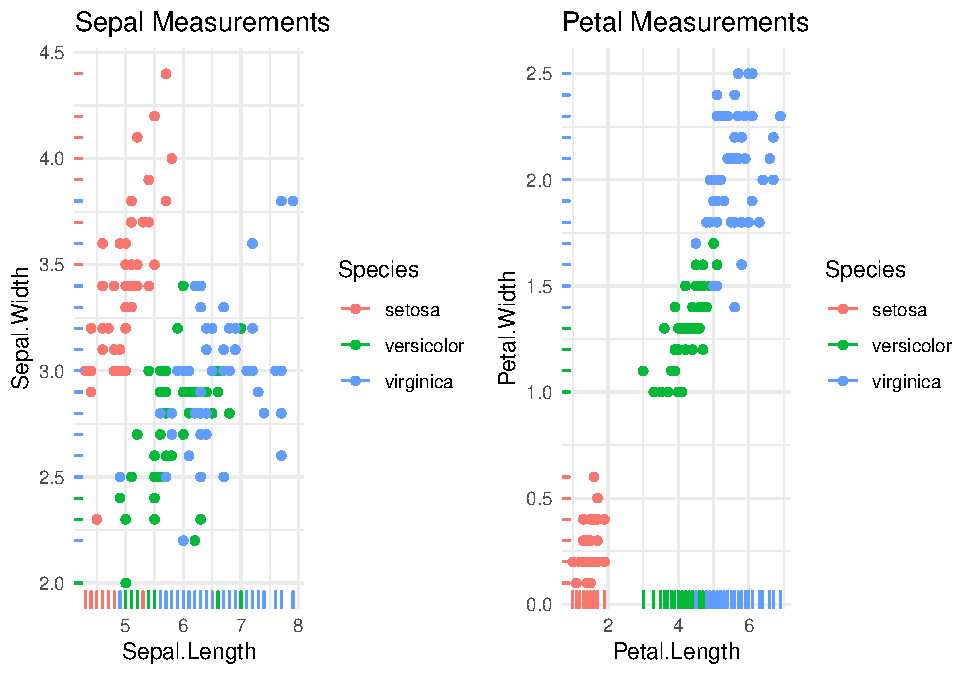
\includegraphics{assessment-1_files/figure-latex/unnamed-chunk-1-1.pdf}

\begin{enumerate}
\def\labelenumi{\arabic{enumi}.}
\tightlist
\item
  Split the data set into a training and a test set with the ratio of
  7:3. (1 mark)
\end{enumerate}

\begin{Shaded}
\begin{Highlighting}[]
\KeywordTok{set.seed}\NormalTok{(}\DecValTok{223}\NormalTok{)}
\NormalTok{iris <-}\StringTok{ }\NormalTok{iris[}\KeywordTok{sample}\NormalTok{(}\DecValTok{1}\OperatorTok{:}\KeywordTok{nrow}\NormalTok{(iris),}\KeywordTok{nrow}\NormalTok{(iris)),]}
\CommentTok{# create  training and testing subsets:}
\NormalTok{train.index =}\StringTok{ }\DecValTok{1}\OperatorTok{:}\DecValTok{105}
\NormalTok{train.data <-}\StringTok{ }\NormalTok{iris[train.index, }\DecValTok{-5}\NormalTok{] }\CommentTok{# grab the first 105 records, leave out the species (last column)}
\NormalTok{train.label <-}\StringTok{ }\NormalTok{iris[train.index, }\DecValTok{5}\NormalTok{]}
\NormalTok{test.data <-}\StringTok{ }\NormalTok{iris[}\OperatorTok{-}\NormalTok{train.index, }\DecValTok{-5}\NormalTok{] }\CommentTok{# grab the last 45 records, leave out the species (last column)}
\NormalTok{test.label <-}\StringTok{ }\NormalTok{iris[}\OperatorTok{-}\NormalTok{train.index, }\DecValTok{5}\NormalTok{]}
\end{Highlighting}
\end{Shaded}

\begin{enumerate}
\def\labelenumi{\arabic{enumi}.}
\setcounter{enumi}{1}
\tightlist
\item
  Implement a KNN classifier. (5 marks)
\end{enumerate}

\begin{Shaded}
\begin{Highlighting}[]
\CommentTok{# define a function that calculates the majority votes (or mode!)}
\NormalTok{majority <-}\StringTok{ }\ControlFlowTok{function}\NormalTok{(x) \{}
\NormalTok{   uniqx <-}\StringTok{ }\KeywordTok{unique}\NormalTok{(x)}
\NormalTok{   uniqx[}\KeywordTok{which.max}\NormalTok{(}\KeywordTok{tabulate}\NormalTok{(}\KeywordTok{match}\NormalTok{(x, uniqx)))]}
\NormalTok{\}}

\CommentTok{#create Knn function using Euclidean distance }
\NormalTok{knn1 <-}\StringTok{ }\ControlFlowTok{function}\NormalTok{(train.data, train.label, test.data, }\DataTypeTok{K=}\NormalTok{k, }\DataTypeTok{distance =} \StringTok{'euclidean'}\NormalTok{)\{}
\NormalTok{    train.len <-}\StringTok{ }\KeywordTok{nrow}\NormalTok{(train.data)}
\NormalTok{    test.len <-}\StringTok{ }\KeywordTok{nrow}\NormalTok{(test.data)}
\NormalTok{    dist <-}\StringTok{ }\KeywordTok{as.matrix}\NormalTok{(}\KeywordTok{dist}\NormalTok{(}\KeywordTok{rbind}\NormalTok{(test.data, train.data), }\DataTypeTok{method=}\NormalTok{ distance))[}\DecValTok{1}\OperatorTok{:}\NormalTok{test.len, (test.len}\OperatorTok{+}\DecValTok{1}\NormalTok{)}\OperatorTok{:}\NormalTok{(test.len}\OperatorTok{+}\NormalTok{train.len)]}
    \ControlFlowTok{for}\NormalTok{ (i }\ControlFlowTok{in} \DecValTok{1}\OperatorTok{:}\NormalTok{test.len)\{}
\NormalTok{        nn <-}\StringTok{ }\KeywordTok{as.data.frame}\NormalTok{(}\KeywordTok{sort}\NormalTok{(dist[i,], }\DataTypeTok{index.return =} \OtherTok{TRUE}\NormalTok{))[}\DecValTok{1}\OperatorTok{:}\NormalTok{K,}\DecValTok{2}\NormalTok{]}
\NormalTok{        test.label[i]<-}\StringTok{ }\NormalTok{(}\KeywordTok{majority}\NormalTok{(train.label[nn]))}
\NormalTok{    \}}
    \KeywordTok{return}\NormalTok{ (test.label)}
\NormalTok{\}}
\end{Highlighting}
\end{Shaded}

\begin{Shaded}
\begin{Highlighting}[]
\CommentTok{#create Knn function using Manhattan distance }
\NormalTok{knn2 <-}\StringTok{ }\ControlFlowTok{function}\NormalTok{(train.data, train.label, test.data, }\DataTypeTok{K=}\NormalTok{k, }\DataTypeTok{distance =} \StringTok{'manhattan'}\NormalTok{)\{}
\NormalTok{    train.len <-}\StringTok{ }\KeywordTok{nrow}\NormalTok{(train.data)}
\NormalTok{    test.len <-}\StringTok{ }\KeywordTok{nrow}\NormalTok{(test.data)}
\NormalTok{    dist <-}\StringTok{ }\KeywordTok{as.matrix}\NormalTok{(}\KeywordTok{dist}\NormalTok{(}\KeywordTok{rbind}\NormalTok{(test.data, train.data), }\DataTypeTok{method=}\NormalTok{ distance))[}\DecValTok{1}\OperatorTok{:}\NormalTok{test.len, (test.len}\OperatorTok{+}\DecValTok{1}\NormalTok{)}\OperatorTok{:}\NormalTok{(test.len}\OperatorTok{+}\NormalTok{train.len)]}
    \ControlFlowTok{for}\NormalTok{ (i }\ControlFlowTok{in} \DecValTok{1}\OperatorTok{:}\NormalTok{test.len)\{}
\NormalTok{        nn <-}\StringTok{ }\KeywordTok{as.data.frame}\NormalTok{(}\KeywordTok{sort}\NormalTok{(dist[i,], }\DataTypeTok{index.return =} \OtherTok{TRUE}\NormalTok{))[}\DecValTok{1}\OperatorTok{:}\NormalTok{K,}\DecValTok{2}\NormalTok{]}
\NormalTok{        test.label[i]<-}\StringTok{ }\NormalTok{(}\KeywordTok{majority}\NormalTok{(train.label[nn]))}
\NormalTok{    \}}
    \KeywordTok{return}\NormalTok{ (test.label)}
\NormalTok{\}}
\end{Highlighting}
\end{Shaded}

\begin{Shaded}
\begin{Highlighting}[]
\CommentTok{#create Knn function using Canberra distance }
\NormalTok{knn3 <-}\StringTok{ }\ControlFlowTok{function}\NormalTok{(train.data, train.label, test.data, }\DataTypeTok{K=}\NormalTok{k, }\DataTypeTok{distance =} \StringTok{'canberra'}\NormalTok{)\{}
\NormalTok{    train.len <-}\StringTok{ }\KeywordTok{nrow}\NormalTok{(train.data)}
\NormalTok{    test.len <-}\StringTok{ }\KeywordTok{nrow}\NormalTok{(test.data)}
\NormalTok{    dist <-}\StringTok{ }\KeywordTok{as.matrix}\NormalTok{(}\KeywordTok{dist}\NormalTok{(}\KeywordTok{rbind}\NormalTok{(test.data, train.data), }\DataTypeTok{method=}\NormalTok{ distance))[}\DecValTok{1}\OperatorTok{:}\NormalTok{test.len, (test.len}\OperatorTok{+}\DecValTok{1}\NormalTok{)}\OperatorTok{:}\NormalTok{(test.len}\OperatorTok{+}\NormalTok{train.len)]}
    \ControlFlowTok{for}\NormalTok{ (i }\ControlFlowTok{in} \DecValTok{1}\OperatorTok{:}\NormalTok{test.len)\{}
\NormalTok{        nn <-}\StringTok{ }\KeywordTok{as.data.frame}\NormalTok{(}\KeywordTok{sort}\NormalTok{(dist[i,], }\DataTypeTok{index.return =} \OtherTok{TRUE}\NormalTok{))[}\DecValTok{1}\OperatorTok{:}\NormalTok{K,}\DecValTok{2}\NormalTok{]}
\NormalTok{        test.label[i]<-}\StringTok{ }\NormalTok{(}\KeywordTok{majority}\NormalTok{(train.label[nn]))}
\NormalTok{    \}}
    \KeywordTok{return}\NormalTok{ (test.label)}
\NormalTok{\}}
\end{Highlighting}
\end{Shaded}

\begin{Shaded}
\begin{Highlighting}[]
\CommentTok{#create Knn function using Minkowski distance }
\NormalTok{knn4 <-}\StringTok{ }\ControlFlowTok{function}\NormalTok{(train.data, train.label, test.data, }\DataTypeTok{K=}\NormalTok{k, }\DataTypeTok{distance =} \StringTok{'minkowski'}\NormalTok{)\{}
\NormalTok{    train.len <-}\StringTok{ }\KeywordTok{nrow}\NormalTok{(train.data)}
\NormalTok{    test.len <-}\StringTok{ }\KeywordTok{nrow}\NormalTok{(test.data)}
\NormalTok{    dist <-}\StringTok{ }\KeywordTok{as.matrix}\NormalTok{(}\KeywordTok{dist}\NormalTok{(}\KeywordTok{rbind}\NormalTok{(test.data, train.data), }\DataTypeTok{method=}\NormalTok{ distance))[}\DecValTok{1}\OperatorTok{:}\NormalTok{test.len, (test.len}\OperatorTok{+}\DecValTok{1}\NormalTok{)}\OperatorTok{:}\NormalTok{(test.len}\OperatorTok{+}\NormalTok{train.len)]}
    \ControlFlowTok{for}\NormalTok{ (i }\ControlFlowTok{in} \DecValTok{1}\OperatorTok{:}\NormalTok{test.len)\{}
\NormalTok{        nn <-}\StringTok{ }\KeywordTok{as.data.frame}\NormalTok{(}\KeywordTok{sort}\NormalTok{(dist[i,], }\DataTypeTok{index.return =} \OtherTok{TRUE}\NormalTok{))[}\DecValTok{1}\OperatorTok{:}\NormalTok{K,}\DecValTok{2}\NormalTok{]}
\NormalTok{        test.label[i]<-}\StringTok{ }\NormalTok{(}\KeywordTok{majority}\NormalTok{(train.label[nn]))}
\NormalTok{    \}}
    \KeywordTok{return}\NormalTok{ (test.label)}
\NormalTok{\}}
\end{Highlighting}
\end{Shaded}

\begin{enumerate}
\def\labelenumi{\arabic{enumi}.}
\setcounter{enumi}{2}
\tightlist
\item
  Investigate the impact of different K (from 1 to 6) values on the
  model performance (ACC) and the impact of different distance
  measurements (euclidean, manhattan, canberra, and minkowski) on the
  model performance (ACC). Visualize and discuss your findings. (14
  marks)
\end{enumerate}

\begin{Shaded}
\begin{Highlighting}[]
\CommentTok{# calculate the train and test missclassification rates for K in 1:6 for each distance }
\NormalTok{miss.Eu <-}\StringTok{ }\KeywordTok{data.frame}\NormalTok{(}\StringTok{'K'}\NormalTok{=}\DecValTok{1}\OperatorTok{:}\DecValTok{6}\NormalTok{, }\StringTok{'train'}\NormalTok{=}\KeywordTok{rep}\NormalTok{(}\DecValTok{0}\NormalTok{,}\DecValTok{6}\NormalTok{), }\StringTok{'test'}\NormalTok{=}\KeywordTok{rep}\NormalTok{(}\DecValTok{0}\NormalTok{,}\DecValTok{6}\NormalTok{))}
\ControlFlowTok{for}\NormalTok{ (k }\ControlFlowTok{in} \DecValTok{1}\OperatorTok{:}\DecValTok{6}\NormalTok{)\{}
\NormalTok{    miss.Eu[k,}\StringTok{'train'}\NormalTok{] <-}\StringTok{ }\KeywordTok{sum}\NormalTok{(}\KeywordTok{knn1}\NormalTok{(train.data, train.label, train.data, }\DataTypeTok{K=}\NormalTok{k) }\OperatorTok{==}\StringTok{ }\NormalTok{train.label)}\OperatorTok{/}\KeywordTok{nrow}\NormalTok{(train.data)}\OperatorTok{*}\DecValTok{100}
\NormalTok{    miss.Eu[k,}\StringTok{'test'}\NormalTok{] <-}\StringTok{  }\KeywordTok{sum}\NormalTok{(}\KeywordTok{knn1}\NormalTok{(train.data, train.label, test.data, }\DataTypeTok{K=}\NormalTok{k)  }\OperatorTok{==}\StringTok{ }\NormalTok{test.label)}\OperatorTok{/}\KeywordTok{nrow}\NormalTok{(test.data)}\OperatorTok{*}\DecValTok{100}
\NormalTok{\}}


\NormalTok{miss.Man <-}\StringTok{ }\KeywordTok{data.frame}\NormalTok{(}\StringTok{'K'}\NormalTok{=}\DecValTok{1}\OperatorTok{:}\DecValTok{6}\NormalTok{, }\StringTok{'train'}\NormalTok{=}\KeywordTok{rep}\NormalTok{(}\DecValTok{0}\NormalTok{,}\DecValTok{6}\NormalTok{), }\StringTok{'test'}\NormalTok{=}\KeywordTok{rep}\NormalTok{(}\DecValTok{0}\NormalTok{,}\DecValTok{6}\NormalTok{))}
\ControlFlowTok{for}\NormalTok{ (k }\ControlFlowTok{in} \DecValTok{1}\OperatorTok{:}\DecValTok{6}\NormalTok{)\{}
\NormalTok{    miss.Man[k,}\StringTok{'train'}\NormalTok{] <-}\StringTok{ }\KeywordTok{sum}\NormalTok{(}\KeywordTok{knn2}\NormalTok{(train.data, train.label, train.data, }\DataTypeTok{K=}\NormalTok{k) }\OperatorTok{==}\StringTok{ }\NormalTok{train.label)}\OperatorTok{/}\KeywordTok{nrow}\NormalTok{(train.data)}\OperatorTok{*}\DecValTok{100}
\NormalTok{    miss.Man[k,}\StringTok{'test'}\NormalTok{] <-}\StringTok{  }\KeywordTok{sum}\NormalTok{(}\KeywordTok{knn2}\NormalTok{(train.data, train.label, test.data, }\DataTypeTok{K=}\NormalTok{k)  }\OperatorTok{==}\StringTok{ }\NormalTok{test.label)}\OperatorTok{/}\KeywordTok{nrow}\NormalTok{(test.data)}\OperatorTok{*}\DecValTok{100}
\NormalTok{\}}

\NormalTok{miss.Can <-}\StringTok{ }\KeywordTok{data.frame}\NormalTok{(}\StringTok{'K'}\NormalTok{=}\DecValTok{1}\OperatorTok{:}\DecValTok{6}\NormalTok{, }\StringTok{'train'}\NormalTok{=}\KeywordTok{rep}\NormalTok{(}\DecValTok{0}\NormalTok{,}\DecValTok{6}\NormalTok{), }\StringTok{'test'}\NormalTok{=}\KeywordTok{rep}\NormalTok{(}\DecValTok{0}\NormalTok{,}\DecValTok{6}\NormalTok{))}
\ControlFlowTok{for}\NormalTok{ (k }\ControlFlowTok{in} \DecValTok{1}\OperatorTok{:}\DecValTok{6}\NormalTok{)\{}
\NormalTok{    miss.Can[k,}\StringTok{'train'}\NormalTok{] <-}\StringTok{ }\KeywordTok{sum}\NormalTok{(}\KeywordTok{knn3}\NormalTok{(train.data, train.label, train.data, }\DataTypeTok{K=}\NormalTok{k) }\OperatorTok{==}\StringTok{ }\NormalTok{train.label)}\OperatorTok{/}\KeywordTok{nrow}\NormalTok{(train.data)}\OperatorTok{*}\DecValTok{100}
\NormalTok{    miss.Can[k,}\StringTok{'test'}\NormalTok{] <-}\StringTok{  }\KeywordTok{sum}\NormalTok{(}\KeywordTok{knn3}\NormalTok{(train.data, train.label, test.data, }\DataTypeTok{K=}\NormalTok{k)  }\OperatorTok{==}\StringTok{ }\NormalTok{test.label)}\OperatorTok{/}\KeywordTok{nrow}\NormalTok{(test.data)}\OperatorTok{*}\DecValTok{100}
\NormalTok{\}}

\NormalTok{miss.Min <-}\StringTok{ }\KeywordTok{data.frame}\NormalTok{(}\StringTok{'K'}\NormalTok{=}\DecValTok{1}\OperatorTok{:}\DecValTok{6}\NormalTok{, }\StringTok{'train'}\NormalTok{=}\KeywordTok{rep}\NormalTok{(}\DecValTok{0}\NormalTok{,}\DecValTok{6}\NormalTok{), }\StringTok{'test'}\NormalTok{=}\KeywordTok{rep}\NormalTok{(}\DecValTok{0}\NormalTok{,}\DecValTok{6}\NormalTok{))}
\ControlFlowTok{for}\NormalTok{ (k }\ControlFlowTok{in} \DecValTok{1}\OperatorTok{:}\DecValTok{6}\NormalTok{)\{}
\NormalTok{    miss.Min[k,}\StringTok{'train'}\NormalTok{] <-}\StringTok{ }\KeywordTok{sum}\NormalTok{(}\KeywordTok{knn4}\NormalTok{(train.data, train.label, train.data, }\DataTypeTok{K=}\NormalTok{k) }\OperatorTok{==}\StringTok{ }\NormalTok{train.label)}\OperatorTok{/}\KeywordTok{nrow}\NormalTok{(train.data)}\OperatorTok{*}\DecValTok{100}
\NormalTok{    miss.Min[k,}\StringTok{'test'}\NormalTok{] <-}\StringTok{  }\KeywordTok{sum}\NormalTok{(}\KeywordTok{knn4}\NormalTok{(train.data, train.label, test.data, }\DataTypeTok{K=}\NormalTok{k)  }\OperatorTok{==}\StringTok{ }\NormalTok{test.label)}\OperatorTok{/}\KeywordTok{nrow}\NormalTok{(test.data)}\OperatorTok{*}\DecValTok{100}
\NormalTok{\}}
\end{Highlighting}
\end{Shaded}

\begin{Shaded}
\begin{Highlighting}[]
\CommentTok{# plot misclassification percentage for train and test data sets}
\NormalTok{miss.m1 <-}\StringTok{ }\KeywordTok{melt}\NormalTok{(miss.Eu, }\DataTypeTok{id=}\StringTok{'K'}\NormalTok{) }\CommentTok{# reshape for visualization}
\KeywordTok{names}\NormalTok{(miss.m1) <-}\StringTok{ }\KeywordTok{c}\NormalTok{(}\StringTok{'K'}\NormalTok{, }\StringTok{'type'}\NormalTok{, }\StringTok{'error'}\NormalTok{)}
\KeywordTok{ggplot}\NormalTok{(}\DataTypeTok{data=}\NormalTok{miss.m1, }\KeywordTok{aes}\NormalTok{(}\DataTypeTok{x=}\NormalTok{ K, }\DataTypeTok{y=}\NormalTok{error, }\DataTypeTok{color=}\NormalTok{type)) }\OperatorTok{+}\StringTok{ }\KeywordTok{geom_line}\NormalTok{() }\OperatorTok{+}
\StringTok{       }\KeywordTok{scale_color_discrete}\NormalTok{(}\DataTypeTok{guide =} \KeywordTok{guide_legend}\NormalTok{(}\DataTypeTok{title =} \OtherTok{NULL}\NormalTok{)) }\OperatorTok{+}\StringTok{ }\KeywordTok{theme_minimal}\NormalTok{() }\OperatorTok{+}
\StringTok{       }\KeywordTok{ggtitle}\NormalTok{(}\StringTok{"Accuracy of KNN Algorithm }\CharTok{\textbackslash{}n}\StringTok{Using Euclidean Distance for K = 1:6"}\NormalTok{) }\OperatorTok{+}\StringTok{ }\KeywordTok{theme}\NormalTok{(}\DataTypeTok{plot.title =} \KeywordTok{element_text}\NormalTok{(}\DataTypeTok{hjust =} \FloatTok{0.5}\NormalTok{))}
\end{Highlighting}
\end{Shaded}

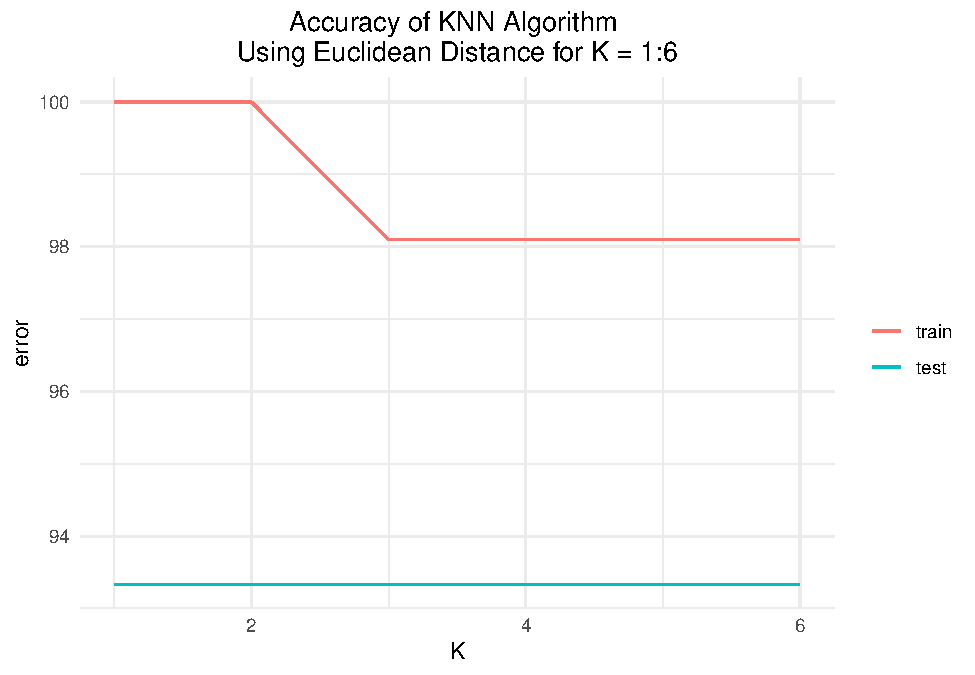
\includegraphics{assessment-1_files/figure-latex/unnamed-chunk-8-1.pdf}

\begin{Shaded}
\begin{Highlighting}[]
\NormalTok{miss.m2 <-}\StringTok{ }\KeywordTok{melt}\NormalTok{(miss.Man, }\DataTypeTok{id=}\StringTok{'K'}\NormalTok{) }\CommentTok{# reshape for visualization}
\KeywordTok{names}\NormalTok{(miss.m2) <-}\StringTok{ }\KeywordTok{c}\NormalTok{(}\StringTok{'K'}\NormalTok{, }\StringTok{'type'}\NormalTok{, }\StringTok{'error'}\NormalTok{)}
\KeywordTok{ggplot}\NormalTok{(}\DataTypeTok{data=}\NormalTok{miss.m2, }\KeywordTok{aes}\NormalTok{(}\DataTypeTok{x=}\NormalTok{K, }\DataTypeTok{y=}\NormalTok{error, }\DataTypeTok{color=}\NormalTok{type)) }\OperatorTok{+}\StringTok{ }\KeywordTok{geom_line}\NormalTok{() }\OperatorTok{+}
\StringTok{       }\KeywordTok{scale_color_discrete}\NormalTok{(}\DataTypeTok{guide =} \KeywordTok{guide_legend}\NormalTok{(}\DataTypeTok{title =} \OtherTok{NULL}\NormalTok{)) }\OperatorTok{+}\StringTok{ }\KeywordTok{theme_minimal}\NormalTok{() }\OperatorTok{+}
\StringTok{       }\KeywordTok{ggtitle}\NormalTok{(}\StringTok{"Accuracy of KNN Algorithm }\CharTok{\textbackslash{}n}\StringTok{Using Manhattan Distance for K = 1:6"}\NormalTok{) }\OperatorTok{+}\StringTok{ }\KeywordTok{theme}\NormalTok{(}\DataTypeTok{plot.title =} \KeywordTok{element_text}\NormalTok{(}\DataTypeTok{hjust =} \FloatTok{0.5}\NormalTok{))}
\end{Highlighting}
\end{Shaded}

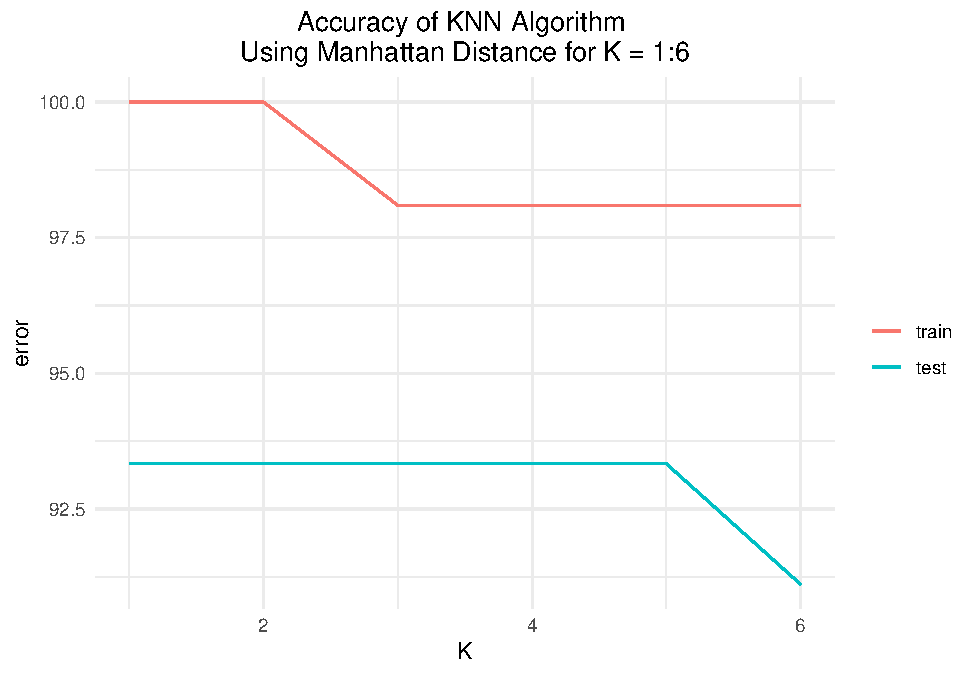
\includegraphics{assessment-1_files/figure-latex/unnamed-chunk-8-2.pdf}

\begin{Shaded}
\begin{Highlighting}[]
\NormalTok{miss.m3 <-}\StringTok{ }\KeywordTok{melt}\NormalTok{(miss.Can, }\DataTypeTok{id=}\StringTok{'K'}\NormalTok{) }\CommentTok{# reshape for visualization}
\KeywordTok{names}\NormalTok{(miss.m3) <-}\StringTok{ }\KeywordTok{c}\NormalTok{(}\StringTok{'K'}\NormalTok{, }\StringTok{'type'}\NormalTok{, }\StringTok{'error'}\NormalTok{)}
\KeywordTok{ggplot}\NormalTok{(}\DataTypeTok{data=}\NormalTok{miss.m3, }\KeywordTok{aes}\NormalTok{(}\DataTypeTok{x=}\NormalTok{K, }\DataTypeTok{y=}\NormalTok{error, }\DataTypeTok{color=}\NormalTok{type)) }\OperatorTok{+}\StringTok{ }\KeywordTok{geom_line}\NormalTok{() }\OperatorTok{+}
\StringTok{       }\KeywordTok{scale_color_discrete}\NormalTok{(}\DataTypeTok{guide =} \KeywordTok{guide_legend}\NormalTok{(}\DataTypeTok{title =} \OtherTok{NULL}\NormalTok{)) }\OperatorTok{+}\StringTok{ }\KeywordTok{theme_minimal}\NormalTok{() }\OperatorTok{+}
\StringTok{       }\KeywordTok{ggtitle}\NormalTok{(}\StringTok{"Accuracy of KNN Algorithm }\CharTok{\textbackslash{}n}\StringTok{Using Canberra Distance for K = 1:6"}\NormalTok{) }\OperatorTok{+}\StringTok{ }\KeywordTok{theme}\NormalTok{(}\DataTypeTok{plot.title =} \KeywordTok{element_text}\NormalTok{(}\DataTypeTok{hjust =} \FloatTok{0.5}\NormalTok{))}
\end{Highlighting}
\end{Shaded}

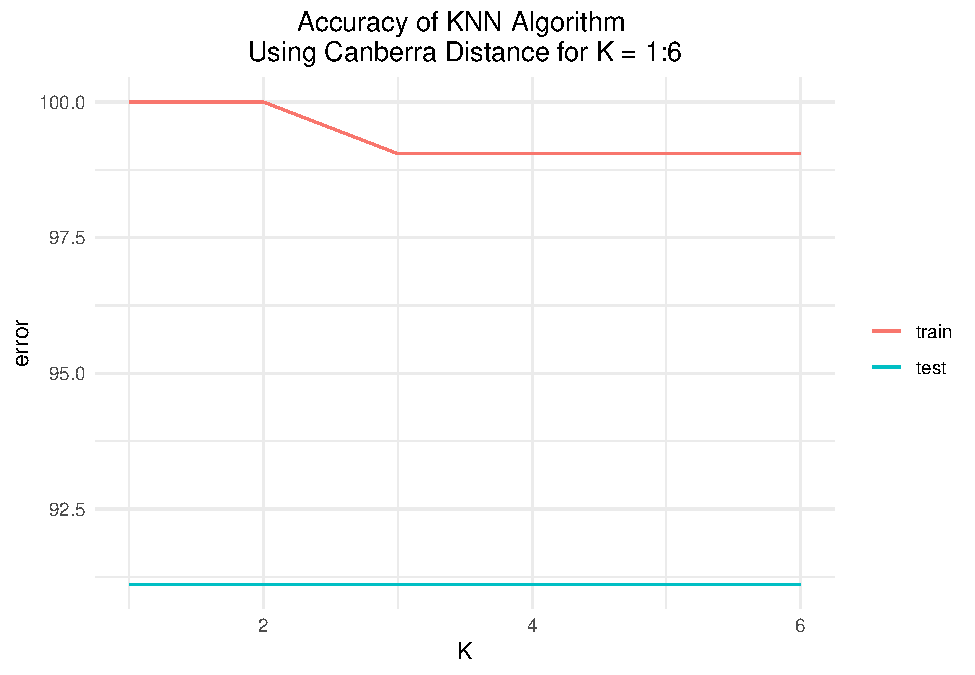
\includegraphics{assessment-1_files/figure-latex/unnamed-chunk-8-3.pdf}

\begin{Shaded}
\begin{Highlighting}[]
\NormalTok{miss.m4 <-}\StringTok{ }\KeywordTok{melt}\NormalTok{(miss.Min, }\DataTypeTok{id=}\StringTok{'K'}\NormalTok{) }\CommentTok{# reshape for visualization}
\KeywordTok{names}\NormalTok{(miss.m4) <-}\StringTok{ }\KeywordTok{c}\NormalTok{(}\StringTok{'K'}\NormalTok{, }\StringTok{'type'}\NormalTok{, }\StringTok{'error'}\NormalTok{)}
\KeywordTok{ggplot}\NormalTok{(}\DataTypeTok{data=}\NormalTok{miss.m4, }\KeywordTok{aes}\NormalTok{(}\DataTypeTok{x=}\NormalTok{K, }\DataTypeTok{y=}\NormalTok{error, }\DataTypeTok{color=}\NormalTok{type)) }\OperatorTok{+}\StringTok{ }\KeywordTok{geom_line}\NormalTok{() }\OperatorTok{+}
\StringTok{       }\KeywordTok{scale_color_discrete}\NormalTok{(}\DataTypeTok{guide =} \KeywordTok{guide_legend}\NormalTok{(}\DataTypeTok{title =} \OtherTok{NULL}\NormalTok{)) }\OperatorTok{+}\StringTok{ }\KeywordTok{theme_minimal}\NormalTok{() }\OperatorTok{+}
\StringTok{       }\KeywordTok{ggtitle}\NormalTok{(}\StringTok{"Accuracy of KNN Algorithm }\CharTok{\textbackslash{}n}\StringTok{Using Minkowski Distance for K = 1:6"}\NormalTok{) }\OperatorTok{+}\StringTok{ }\KeywordTok{theme}\NormalTok{(}\DataTypeTok{plot.title =} \KeywordTok{element_text}\NormalTok{(}\DataTypeTok{hjust =} \FloatTok{0.5}\NormalTok{)) }
\end{Highlighting}
\end{Shaded}

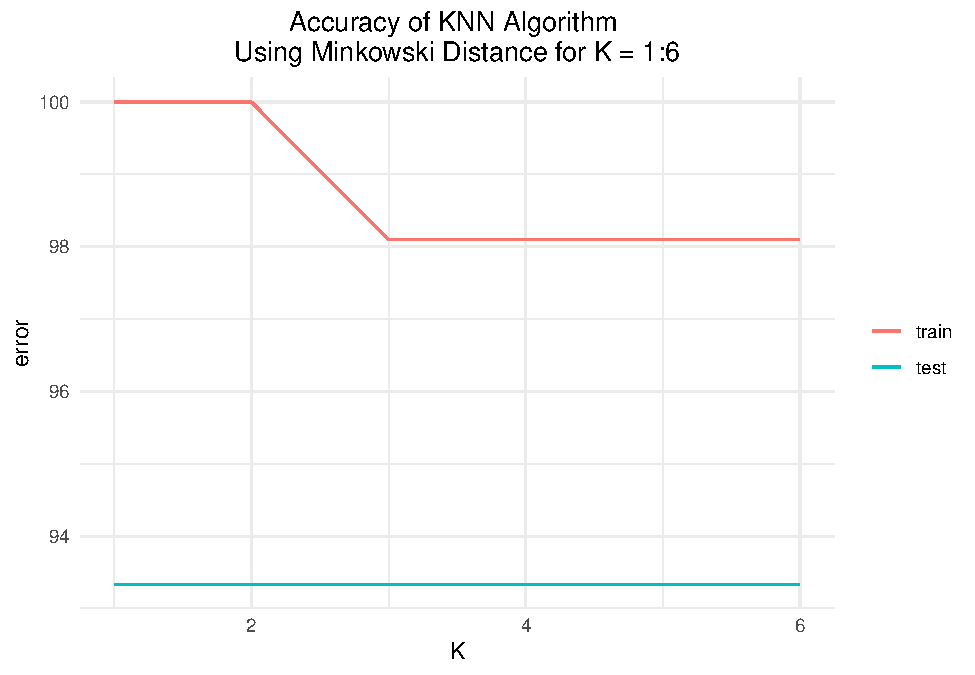
\includegraphics{assessment-1_files/figure-latex/unnamed-chunk-8-4.pdf}
\#\# Question 2 - Linear Regression (35 marks)

In this question you need to implement a linear regression model to
predict health care cost. The data set used in this question can be
found in `insurance.csv'. The data set has 7 features, which are
summarized as below.

\begin{itemize}
\tightlist
\item
  Age: insurance contractor age, years
\item
  Sex: insurance contractor gender, {[}female, male{]}
\item
  BMI: Body mass index, providing an understanding of body, weights that
  are relatively high or low relative to height, objective index of body
  weight (kg / m \^{} 2) using the ratio of height to weight, ideally
  18.5 to 24.9
\item
  Children: number of children covered by health insurance / Number of
  dependents
\item
  Smoker: smoking, {[}yes, no{]}
\item
  Region: the beneficiary's residential area in the US, {[}northeast,
  southeast, southwest, northwest{]}
\item
  Charges: Individual medical costs billed by health insurance, \$
  \#predicted value
\end{itemize}

Specifically, you need to:

\begin{enumerate}
\def\labelenumi{\arabic{enumi}.}
\tightlist
\item
  Perform data pre-processing, including removing invalid data and
  transfromatting the categorical features to numerical features. (4
  marks)
\item
  Split the data set into a training set and a test set, with ratio of
  7:3. (2 mark)
\item
  Implement a linear regression model and train the model with your
  training data. Visualize the parameter updating process, test error
  (RMSE) in each iteration, and cost convergence process. Please be
  advised that built-in models in any realeased R package, like glm, is
  not allowed to use in this question. You can choose your preferred
  learning rate and determine the best iteration number. (8 marks)
\item
  Evaluate your model by calculating the RMSE, and visualizing the
  residuals of test data. Please note that explanation of your residual
  plot is needed. (5 marks)
\item
  Does your model overfit? Which features do you think are not
  significant? Please justify your answers. For example, you can analyze
  the significance of a feature from correlation, variance, etc. (8
  marks)
\item
  Use the glmnet library to biult two linear regression models with
  Lasso and Ridge regularization, respectively. In comparison to your
  model, how well do these two models perform? Do the regularized models
  automatically filter out the less significant features? What are the
  differences of these two models? Please justify your answers. (8
  marks)
\end{enumerate}

\begin{Shaded}
\begin{Highlighting}[]
\NormalTok{data =}\StringTok{ }\KeywordTok{read.csv}\NormalTok{(}\StringTok{'insurance.csv'}\NormalTok{)}
\end{Highlighting}
\end{Shaded}

\emph{1. data pre-processing:} Before the data can be used in any sort
of linear regression, it first must be checked and cleaned of any
missing, invalid or outlier data. Initially all missing values were
removed from the dataset. Then each attribute was checked via a box plot
to check to see if there were any outliers present in the dataset, 9
outliers were found in the \emph{bmi} attribute and were removed from
the data set as they were outside the known range for bmis (12-42). 136
outliers were found in the charges attribute and were also removed from
the dataset. The data was also normalised for the convenience of the
analysis.

\begin{Shaded}
\begin{Highlighting}[]
\CommentTok{##check for missing values }
\NormalTok{data <-}\StringTok{ }\KeywordTok{na.omit}\NormalTok{(data)}

\CommentTok{##check for outliers }
\NormalTok{outliers.age <-}\StringTok{ }\KeywordTok{boxplot.stats}\NormalTok{(data}\OperatorTok{$}\NormalTok{age)}\OperatorTok{$}\NormalTok{out}
\KeywordTok{boxplot}\NormalTok{(data}\OperatorTok{$}\NormalTok{age, }\DataTypeTok{main =} \StringTok{"Age"}\NormalTok{, }\DataTypeTok{boxwex =} \FloatTok{0.1}\NormalTok{)}
\KeywordTok{mtext}\NormalTok{(}\KeywordTok{paste}\NormalTok{(}\StringTok{"Outliers: "}\NormalTok{, }\KeywordTok{paste}\NormalTok{(outliers.age, }\DataTypeTok{collapse =} \StringTok{", "}\NormalTok{)), }\DataTypeTok{cex =} \FloatTok{0.6}\NormalTok{)}
\end{Highlighting}
\end{Shaded}

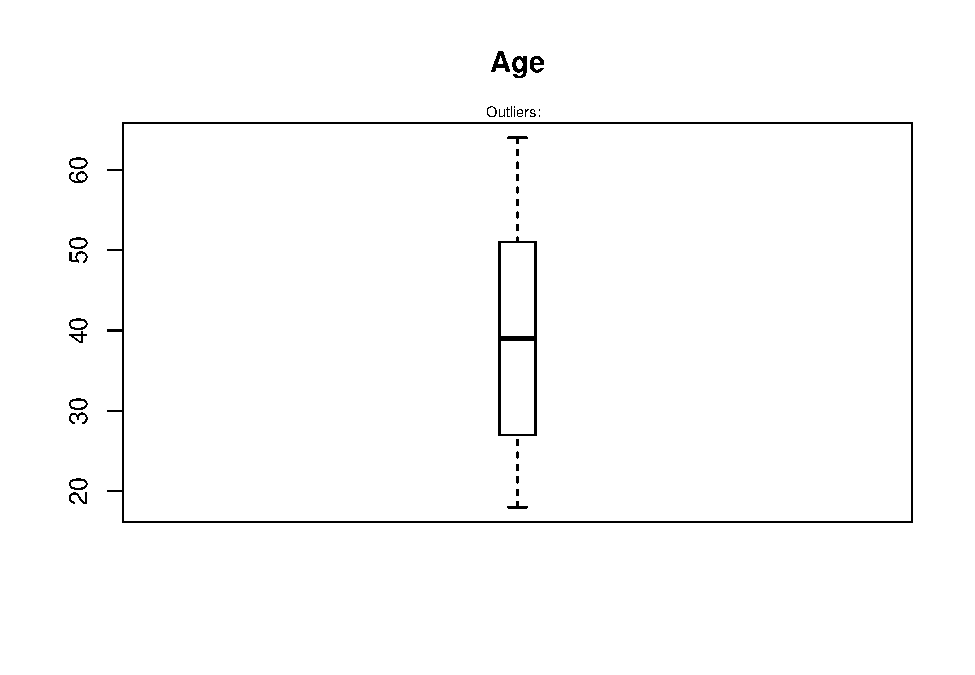
\includegraphics{assessment-1_files/figure-latex/unnamed-chunk-10-1.pdf}

\begin{Shaded}
\begin{Highlighting}[]
\NormalTok{outliers.bmi <-}\StringTok{ }\KeywordTok{boxplot}\NormalTok{(data}\OperatorTok{$}\NormalTok{bmi, }\DataTypeTok{plot =} \OtherTok{FALSE}\NormalTok{)}\OperatorTok{$}\NormalTok{out }\CommentTok{#### appears to be outliers that are unrealistic bmi scores and as such will be removed for being invalid }
\KeywordTok{boxplot}\NormalTok{(data}\OperatorTok{$}\NormalTok{bmi, }\DataTypeTok{main =} \StringTok{"BMI"}\NormalTok{, }\DataTypeTok{boxwex =} \FloatTok{0.1}\NormalTok{)}
\KeywordTok{mtext}\NormalTok{(}\KeywordTok{paste}\NormalTok{(}\StringTok{"Outliers: "}\NormalTok{, }\KeywordTok{paste}\NormalTok{(outliers.bmi, }\DataTypeTok{collapse =} \StringTok{", "}\NormalTok{)), }\DataTypeTok{cex =} \FloatTok{0.6}\NormalTok{)}
\end{Highlighting}
\end{Shaded}

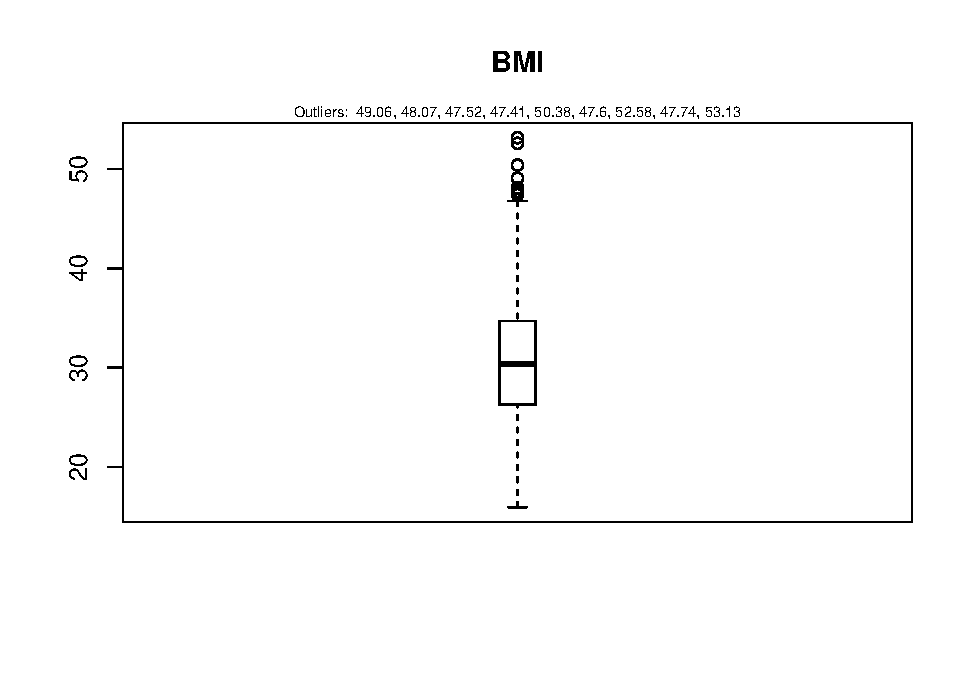
\includegraphics{assessment-1_files/figure-latex/unnamed-chunk-10-2.pdf}

\begin{Shaded}
\begin{Highlighting}[]
\NormalTok{outliers.children <-}\StringTok{ }\KeywordTok{boxplot.stats}\NormalTok{(data}\OperatorTok{$}\NormalTok{children)}\OperatorTok{$}\NormalTok{out}
\KeywordTok{boxplot}\NormalTok{(data}\OperatorTok{$}\NormalTok{children, }\DataTypeTok{main =} \StringTok{"Children"}\NormalTok{, }\DataTypeTok{boxwex =} \FloatTok{0.1}\NormalTok{)}
\KeywordTok{mtext}\NormalTok{(}\KeywordTok{paste}\NormalTok{(}\StringTok{"Outliers: "}\NormalTok{, }\KeywordTok{paste}\NormalTok{(outliers.children, }\DataTypeTok{collapse =} \StringTok{", "}\NormalTok{)), }\DataTypeTok{cex =} \FloatTok{0.6}\NormalTok{)}
\end{Highlighting}
\end{Shaded}

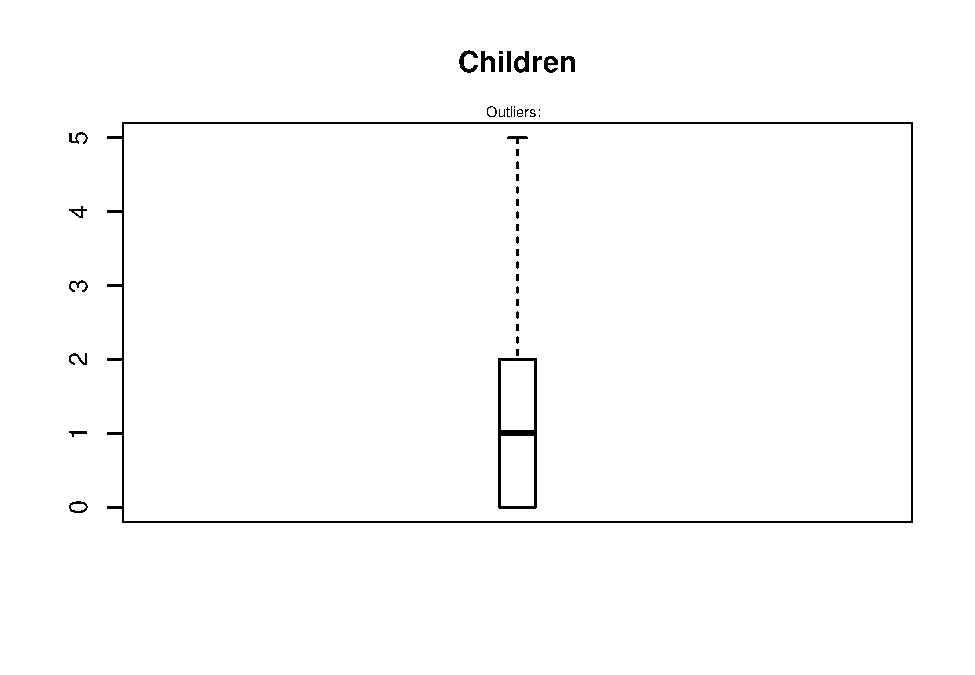
\includegraphics{assessment-1_files/figure-latex/unnamed-chunk-10-3.pdf}

\begin{Shaded}
\begin{Highlighting}[]
\NormalTok{outliers.charges <-}\StringTok{ }\KeywordTok{boxplot.stats}\NormalTok{(data}\OperatorTok{$}\NormalTok{charges)}\OperatorTok{$}\NormalTok{out}
\KeywordTok{boxplot}\NormalTok{(data}\OperatorTok{$}\NormalTok{charges, }\DataTypeTok{main =} \StringTok{"Charges"}\NormalTok{, }\DataTypeTok{boxwex =} \FloatTok{0.1}\NormalTok{)}
\KeywordTok{mtext}\NormalTok{(}\KeywordTok{paste}\NormalTok{(}\StringTok{"Outliers: "}\NormalTok{, }\KeywordTok{paste}\NormalTok{(outliers.charges, }\DataTypeTok{collapse =} \StringTok{", "}\NormalTok{)), }\DataTypeTok{cex =} \FloatTok{0.6}\NormalTok{)}
\end{Highlighting}
\end{Shaded}

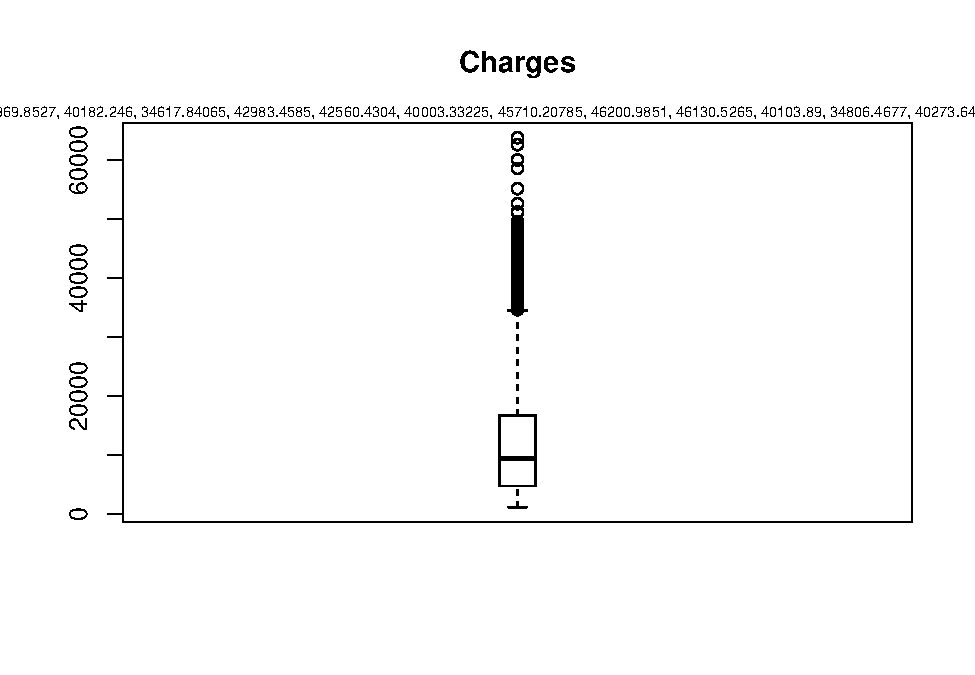
\includegraphics{assessment-1_files/figure-latex/unnamed-chunk-10-4.pdf}

\begin{Shaded}
\begin{Highlighting}[]
\CommentTok{#find which rows contain bmi outliers and remove rows}
\NormalTok{data[}\KeywordTok{which}\NormalTok{(data}\OperatorTok{$}\NormalTok{bmi }\OperatorTok\StringTok{ }\NormalTok{outliers.bmi), ]}
\end{Highlighting}
\end{Shaded}

\begin{verbatim}
##      age    sex   bmi children smoker    region   charges
## 117   58   male 49.06        0     no southeast 11381.325
## 287   46 female 48.07        2     no northeast  9432.925
## 402   47   male 47.52        1     no southeast  8083.920
## 544   54 female 47.41        0    yes southeast 63770.428
## 848   23   male 50.38        1     no southeast  2438.055
## 861   37 female 47.60        2    yes southwest 46113.511
## 1048  22   male 52.58        1    yes southeast 44501.398
## 1089  52   male 47.74        1     no southeast  9748.911
## 1318  18   male 53.13        0     no southeast  1163.463
\end{verbatim}

\begin{Shaded}
\begin{Highlighting}[]
\NormalTok{data <-}\StringTok{ }\NormalTok{data[}\OperatorTok{-}\KeywordTok{which}\NormalTok{(data}\OperatorTok{$}\NormalTok{bmi }\OperatorTok\StringTok{ }\NormalTok{outliers.bmi), ]}

\NormalTok{data[}\KeywordTok{which}\NormalTok{(data}\OperatorTok{$}\NormalTok{charges }\OperatorTok\StringTok{ }\NormalTok{outliers.charges), ]}
\end{Highlighting}
\end{Shaded}

\begin{verbatim}
##      age    sex    bmi children smoker    region  charges
## 15    27   male 42.130        0    yes southeast 39611.76
## 20    30   male 35.300        0    yes southwest 36837.47
## 24    34 female 31.920        1    yes northeast 37701.88
## 30    31   male 36.300        2    yes southwest 38711.00
## 31    22   male 35.600        0    yes southwest 35585.58
## 35    28   male 36.400        1    yes southwest 51194.56
## 39    35   male 36.670        1    yes northeast 39774.28
## 40    60   male 39.900        0    yes southwest 48173.36
## 50    36   male 35.200        1    yes southeast 38709.18
## 54    36   male 34.430        0    yes southeast 37742.58
## 56    58   male 36.955        2    yes northwest 47496.49
## 83    22   male 37.620        1    yes southeast 37165.16
## 85    37 female 34.800        2    yes southwest 39836.52
## 87    57 female 31.160        0    yes northwest 43578.94
## 95    64 female 31.300        2    yes southwest 47291.06
## 110   63   male 35.090        0    yes southeast 47055.53
## 124   44   male 31.350        1    yes northeast 39556.49
## 147   46   male 30.495        3    yes northwest 40720.55
## 159   30   male 35.530        0    yes southeast 36950.26
## 162   18 female 36.850        0    yes southeast 36149.48
## 176   63 female 37.700        0    yes southwest 48824.45
## 186   36   male 41.895        3    yes northeast 43753.34
## 204   27 female 36.080        0    yes southeast 37133.90
## 224   19   male 34.800        0    yes southwest 34779.61
## 241   23 female 36.670        2    yes northeast 38511.63
## 243   55 female 26.800        1     no southwest 35160.13
## 252   63 female 32.200        2    yes southwest 47305.31
## 253   54   male 34.210        2    yes southeast 44260.75
## 255   50   male 31.825        0    yes northeast 41097.16
## 257   56   male 33.630        0    yes northwest 43921.18
## 264   19   male 36.955        0    yes northwest 36219.41
## 266   46   male 42.350        3    yes southeast 46151.12
## 272   50   male 34.200        2    yes southwest 42856.84
## 282   54   male 40.565        3    yes northeast 48549.18
## 289   59 female 36.765        1    yes northeast 47896.79
## 293   25   male 45.540        2    yes southeast 42112.24
## 299   31   male 34.390        3    yes northwest 38746.36
## 313   43   male 35.970        3    yes southeast 42124.52
## 315   27 female 31.400        0    yes southwest 34838.87
## 323   34   male 30.800        0    yes southwest 35491.64
## 328   45   male 36.480        2    yes northwest 42760.50
## 329   64 female 33.800        1    yes southwest 47928.03
## 331   61 female 36.385        1    yes northeast 48517.56
## 339   50   male 32.300        1    yes northeast 41919.10
## 374   26   male 32.900        2    yes southwest 36085.22
## 378   24   male 40.150        0    yes southeast 38126.25
## 382   55   male 30.685        0    yes northeast 42303.69
## 421   64   male 33.880        0    yes southeast 46889.26
## 422   61   male 35.860        0    yes southeast 46599.11
## 423   40   male 32.775        1    yes northeast 39125.33
## 442   33 female 33.500        0    yes southwest 37079.37
## 477   24   male 28.500        0    yes northeast 35147.53
## 489   44 female 38.060        0    yes southeast 48885.14
## 501   29   male 34.400        0    yes southwest 36197.70
## 525   42   male 26.070        1    yes southeast 38245.59
## 531   57   male 42.130        1    yes southeast 48675.52
## 550   43 female 46.200        0    yes southeast 45863.21
## 559   35 female 34.105        3    yes northwest 39983.43
## 570   48   male 40.565        2    yes northwest 45702.02
## 578   31 female 38.095        1    yes northeast 58571.07
## 588   34 female 30.210        1    yes northwest 43943.88
## 610   30   male 37.800        2    yes southwest 39241.44
## 616   47 female 36.630        1    yes southeast 42969.85
## 622   37   male 34.100        4    yes southwest 40182.25
## 624   18   male 33.535        0    yes northeast 34617.84
## 630   44 female 38.950        0    yes northwest 42983.46
## 666   43   male 38.060        2    yes southeast 42560.43
## 668   40 female 32.775        2    yes northwest 40003.33
## 669   62   male 32.015        0    yes northeast 45710.21
## 675   44 female 43.890        2    yes southeast 46200.99
## 678   60   male 31.350        3    yes northwest 46130.53
## 683   39   male 35.300        2    yes southwest 40103.89
## 690   27   male 31.130        1    yes southeast 34806.47
## 698   41   male 35.750        1    yes southeast 40273.65
## 707   51 female 38.060        0    yes southeast 44400.41
## 726   30 female 39.050        3    yes southeast 40932.43
## 737   37 female 38.390        0    yes southeast 40419.02
## 739   23   male 31.730        3    yes northeast 36189.10
## 740   29   male 35.500        2    yes southwest 44585.46
## 743   53   male 34.105        0    yes northeast 43254.42
## 760   18   male 38.170        0    yes southeast 36307.80
## 804   18 female 42.240        0    yes southeast 38792.69
## 820   33 female 35.530        0    yes northwest 55135.40
## 827   56   male 31.790        2    yes southeast 43813.87
## 829   41   male 30.780        3    yes northeast 39597.41
## 843   23 female 32.780        2    yes southeast 36021.01
## 846   60 female 32.450        0    yes southeast 45008.96
## 851   37 female 30.780        0    yes northeast 37270.15
## 853   46 female 35.530        0    yes northeast 42111.66
## 857   48 female 33.110        0    yes southeast 40974.16
## 884   51 female 37.050        3    yes northeast 46255.11
## 894   47   male 38.940        2    yes southeast 44202.65
## 902   60   male 40.920        0    yes southeast 48673.56
## 918   45   male 22.895        0    yes northeast 35069.37
## 948   37   male 34.200        1    yes northeast 39047.29
## 952   51   male 42.900        2    yes southeast 47462.89
## 954   44   male 30.200        2    yes southwest 38998.55
## 957   54   male 30.800        1    yes southeast 41999.52
## 959   43   male 34.960        1    yes northeast 41034.22
## 1013  61 female 33.330        4     no southeast 36580.28
## 1022  22 female 31.020        3    yes southeast 35595.59
## 1023  47   male 36.080        1    yes southeast 42211.14
## 1032  55 female 35.200        0    yes southeast 44423.80
## 1037  22   male 37.070        2    yes southeast 37484.45
## 1038  45 female 30.495        1    yes northwest 39725.52
## 1050  49   male 30.900        0    yes southwest 39727.61
## 1063  59   male 41.140        1    yes southeast 48970.25
## 1071  37   male 37.070        1    yes southeast 39871.70
## 1079  28   male 31.680        0    yes southeast 34672.15
## 1091  47   male 36.190        0    yes southeast 41676.08
## 1097  51 female 34.960        2    yes northeast 44641.20
## 1112  38   male 38.390        3    yes southeast 41949.24
## 1118  25   male 33.330        2    yes southeast 36124.57
## 1119  33   male 35.750        1    yes southeast 38282.75
## 1123  53 female 36.860        3    yes northwest 46661.44
## 1125  23 female 42.750        1    yes northeast 40904.20
## 1140  19 female 32.490        0    yes northwest 36898.73
## 1147  60   male 32.800        0    yes southwest 52590.83
## 1153  43 female 32.560        3    yes southeast 40941.29
## 1157  19   male 44.880        0    yes southeast 39722.75
## 1187  20   male 35.625        3    yes northwest 37465.34
## 1207  59 female 34.800        2     no southwest 36910.61
## 1208  36   male 33.400        2    yes southwest 38415.47
## 1219  46 female 34.600        1    yes southwest 41661.60
## 1231  52   male 34.485        3    yes northwest 60021.40
## 1241  52   male 41.800        2    yes southeast 47269.85
## 1242  64   male 36.960        2    yes southeast 49577.66
## 1250  32   male 33.630        1    yes northeast 37607.53
## 1285  61   male 36.300        1    yes southwest 47403.88
## 1289  20   male 39.400        2    yes southwest 38344.57
## 1292  19   male 34.900        0    yes southwest 34828.65
## 1301  45   male 30.360        0    yes southeast 62592.87
## 1302  62   male 30.875        3    yes northwest 46718.16
## 1304  43   male 27.800        0    yes southwest 37829.72
## 1314  19 female 34.700        2    yes southwest 36397.58
## 1324  42 female 40.370        2    yes southeast 43896.38
\end{verbatim}

\begin{Shaded}
\begin{Highlighting}[]
\NormalTok{data <-}\StringTok{ }\NormalTok{data[}\OperatorTok{-}\KeywordTok{which}\NormalTok{(data}\OperatorTok{$}\NormalTok{charges }\OperatorTok\StringTok{ }\NormalTok{outliers.charges), ]}

\CommentTok{#check to make sure outliers were removed  }
\NormalTok{data[}\KeywordTok{which}\NormalTok{(data}\OperatorTok{$}\NormalTok{charges }\OperatorTok\StringTok{ }\NormalTok{outliers.charges), ]}
\end{Highlighting}
\end{Shaded}

\begin{verbatim}
## [1] age      sex      bmi      children smoker   region   charges 
## <0 rows> (or 0-length row.names)
\end{verbatim}

\begin{Shaded}
\begin{Highlighting}[]
\NormalTok{data[}\KeywordTok{which}\NormalTok{(data}\OperatorTok{$}\NormalTok{charges }\OperatorTok\StringTok{ }\NormalTok{outliers.charges), ]}
\end{Highlighting}
\end{Shaded}

\begin{verbatim}
## [1] age      sex      bmi      children smoker   region   charges 
## <0 rows> (or 0-length row.names)
\end{verbatim}

\begin{Shaded}
\begin{Highlighting}[]
\CommentTok{## transformatting categorical data into numerical }
\NormalTok{data}\OperatorTok{$}\NormalTok{sex <-}\StringTok{ }\KeywordTok{as.numeric}\NormalTok{(data}\OperatorTok{$}\NormalTok{sex)}
\NormalTok{data}\OperatorTok{$}\NormalTok{smoker <-}\StringTok{ }\KeywordTok{as.numeric}\NormalTok{(data}\OperatorTok{$}\NormalTok{smoker)}
\NormalTok{data}\OperatorTok{$}\NormalTok{region <-}\StringTok{ }\KeywordTok{as.numeric}\NormalTok{(data}\OperatorTok{$}\NormalTok{smoker)}
\end{Highlighting}
\end{Shaded}

2: split data into training and test datasets The data was split into
training and test datasets with a ratio of 7:3

\begin{Shaded}
\begin{Highlighting}[]
\CommentTok{# set seed for replication of results }
\KeywordTok{set.seed}\NormalTok{(}\DecValTok{334}\NormalTok{)}

\CommentTok{#create function to normalise the data to aid in creating the linear model }
\NormalTok{normalize <-}\StringTok{ }\ControlFlowTok{function}\NormalTok{(x)\{}
\NormalTok{  num <-}\StringTok{ }\NormalTok{x }\OperatorTok{-}\StringTok{ }\KeywordTok{min}\NormalTok{(x)}
\NormalTok{  denom <-}\StringTok{ }\KeywordTok{max}\NormalTok{(x) }\OperatorTok{-}\StringTok{ }\KeywordTok{min}\NormalTok{(x)}
  \KeywordTok{return}\NormalTok{(num}\OperatorTok{/}\NormalTok{denom)}
\NormalTok{\}}

\CommentTok{#normalise the data }
\NormalTok{normdata <-}\StringTok{ }\KeywordTok{as.data.frame}\NormalTok{(}\KeywordTok{lapply}\NormalTok{(data, normalize))}

\CommentTok{# divide data into training and testing sets}
\NormalTok{D <-}\StringTok{ }\DecValTok{7}
\NormalTok{N <-}\StringTok{ }\DecValTok{1193}
\NormalTok{train.len <-}\StringTok{ }\DecValTok{835}
\NormalTok{train.index <-}\StringTok{ }\KeywordTok{sample}\NormalTok{(}\DecValTok{1}\OperatorTok{:}\NormalTok{N,train.len)}
\NormalTok{train.data <-}\StringTok{ }\NormalTok{normdata[train.index,  }\DecValTok{1}\OperatorTok{:}\NormalTok{D]}
\NormalTok{test.data <-}\StringTok{ }\NormalTok{normdata[}\OperatorTok{-}\NormalTok{train.index, }\DecValTok{1}\OperatorTok{:}\NormalTok{D]}
\end{Highlighting}
\end{Shaded}

\begin{enumerate}
\def\labelenumi{\arabic{enumi}.}
\setcounter{enumi}{2}
\tightlist
\item
  Implement a linear regression model and train the model with your
  training data. Visualize the parameter updating process, test error
  (RMSE) in each iteration, and cost convergence process. Please be
  advised that built-in models in any realeased R package, like glm, is
  not allowed to use in this question. You can choose your preferred
  learning rate and determine the best iteration number.
\end{enumerate}

\begin{Shaded}
\begin{Highlighting}[]
\CommentTok{###create function to calculate coefficients for linear model using charges as the response variable}
\CommentTok{#x: matrix input for the model}
\CommentTok{#y: a matrix for the target for the model}
\CommentTok{#alpha: learning rate for the algorithum}
\CommentTok{#epsilon: value used to test the while loop. once the difference in the cost function between iteration is less than this value the while loop will stop }
\NormalTok{GradD <-}\StringTok{ }\ControlFlowTok{function}\NormalTok{(x, y, }\DataTypeTok{alpha =} \FloatTok{0.006}\NormalTok{, }\DataTypeTok{epsilon =} \DecValTok{10}\OperatorTok{^-}\DecValTok{10}\NormalTok{)\{}
\NormalTok{  iter <-}\StringTok{ }\DecValTok{0}
\NormalTok{  i <-}\StringTok{ }\DecValTok{0}
\NormalTok{  x <-}\StringTok{ }\KeywordTok{cbind}\NormalTok{(}\KeywordTok{rep}\NormalTok{(}\DecValTok{1}\NormalTok{,}\KeywordTok{nrow}\NormalTok{(x)), x)}
\NormalTok{  theta <-}\StringTok{ }\KeywordTok{matrix}\NormalTok{(}\KeywordTok{c}\NormalTok{(}\DecValTok{1}\NormalTok{,}\DecValTok{1}\NormalTok{),}\KeywordTok{ncol}\NormalTok{(x),}\DecValTok{1}\NormalTok{)}
\NormalTok{  cost <-}\StringTok{ }\NormalTok{(}\DecValTok{1}\OperatorTok{/}\NormalTok{(}\DecValTok{2}\OperatorTok{*}\KeywordTok{nrow}\NormalTok{(x))) }\OperatorTok{*}\StringTok{ }\KeywordTok{t}\NormalTok{(x }\OperatorTok\StringTok{ }\NormalTok{theta }\OperatorTok{-}\StringTok{ }\NormalTok{y) }\OperatorTok\StringTok{ }\NormalTok{(x }\OperatorTok\StringTok{ }\NormalTok{theta }\OperatorTok{-}\StringTok{ }\NormalTok{y)}
\NormalTok{  delta <-}\StringTok{ }\DecValTok{1}
  \ControlFlowTok{while}\NormalTok{(delta }\OperatorTok{>}\StringTok{ }\NormalTok{epsilon)\{}
\NormalTok{    i <-}\StringTok{ }\NormalTok{i }\OperatorTok{+}\StringTok{ }\DecValTok{1}
\NormalTok{    theta <-}\StringTok{ }\NormalTok{theta }\OperatorTok{-}\StringTok{ }\NormalTok{(alpha }\OperatorTok{/}\StringTok{ }\KeywordTok{nrow}\NormalTok{(x)) }\OperatorTok{*}\StringTok{ }\NormalTok{(}\KeywordTok{t}\NormalTok{(x) }\OperatorTok\StringTok{ }\NormalTok{(x }\OperatorTok\StringTok{ }\NormalTok{theta }\OperatorTok{-}\StringTok{ }\NormalTok{y))}
\NormalTok{    cval <-}\StringTok{ }\NormalTok{(}\DecValTok{1}\OperatorTok{/}\NormalTok{(}\DecValTok{2}\OperatorTok{*}\KeywordTok{nrow}\NormalTok{(x))) }\OperatorTok{*}\StringTok{ }\KeywordTok{t}\NormalTok{(x }\OperatorTok\StringTok{ }\NormalTok{theta }\OperatorTok{-}\StringTok{ }\NormalTok{y) }\OperatorTok\StringTok{ }\NormalTok{(x }\OperatorTok\StringTok{ }\NormalTok{theta }\OperatorTok{-}\StringTok{ }\NormalTok{y)}
\NormalTok{    cost <-}\StringTok{ }\KeywordTok{append}\NormalTok{(cost, cval)}
\NormalTok{    delta <-}\StringTok{ }\KeywordTok{abs}\NormalTok{(cost[i}\OperatorTok{+}\DecValTok{1}\NormalTok{] }\OperatorTok{-}\StringTok{ }\NormalTok{cost[i])}
    \ControlFlowTok{if}\NormalTok{((cost[i}\OperatorTok{+}\DecValTok{1}\NormalTok{] }\OperatorTok{-}\StringTok{ }\NormalTok{cost[i]) }\OperatorTok{>}\StringTok{ }\DecValTok{0}\NormalTok{)\{}
      \KeywordTok{print}\NormalTok{(}\StringTok{"The cost is increasing.  Try reducing alpha."}\NormalTok{)}
      \KeywordTok{return}\NormalTok{()}
\NormalTok{    \}}
\NormalTok{    iter <-}\StringTok{ }\KeywordTok{append}\NormalTok{(iter, i)}
\NormalTok{  \}}
  \KeywordTok{print}\NormalTok{(}\KeywordTok{sprintf}\NormalTok{(}\StringTok{"Completed in %i iterations."}\NormalTok{, i))}
  \KeywordTok{return}\NormalTok{(theta)}
\NormalTok{\}}
\end{Highlighting}
\end{Shaded}

\begin{Shaded}
\begin{Highlighting}[]
\CommentTok{#create x and y variables using insurance data }
\NormalTok{x <-}\StringTok{ }\KeywordTok{as.matrix}\NormalTok{(train.data[}\DecValTok{1}\OperatorTok{:}\DecValTok{6}\NormalTok{])}
\NormalTok{y <-}\StringTok{ }\KeywordTok{as.matrix}\NormalTok{(train.data}\OperatorTok{$}\NormalTok{charges)}

\CommentTok{#run gradient descent function }
\NormalTok{theta <-}\StringTok{ }\KeywordTok{GradD}\NormalTok{(x, y, }\DataTypeTok{alpha =} \FloatTok{0.1}\NormalTok{, }\DataTypeTok{epsilon =} \DecValTok{10}\OperatorTok{^-}\DecValTok{10}\NormalTok{)}
\end{Highlighting}
\end{Shaded}

\begin{verbatim}
## Warning in matrix(c(1, 1), ncol(x), 1): data length [2] is not a sub-multiple or
## multiple of the number of rows [7]
\end{verbatim}

\begin{verbatim}
## [1] "Completed in 2258 iterations."
\end{verbatim}

\begin{Shaded}
\begin{Highlighting}[]
\NormalTok{theta}
\end{Highlighting}
\end{Shaded}

\begin{verbatim}
##                  [,1]
##           0.037326954
## age       0.319717313
## sex      -0.006083227
## bmi       0.049320218
## children  0.056182832
## smoker    0.224081471
## region    0.224081471
\end{verbatim}

\begin{Shaded}
\begin{Highlighting}[]
\KeywordTok{View}\NormalTok{(theta)}
\end{Highlighting}
\end{Shaded}

\begin{enumerate}
\def\labelenumi{\arabic{enumi}.}
\setcounter{enumi}{3}
\tightlist
\item
  Evaluate your model by calculating the RMSE, and visualizing the
  residuals of test data. Please note that explanation of your residual
  plot is needed. (5 marks)
\end{enumerate}

\begin{Shaded}
\begin{Highlighting}[]
\CommentTok{#create the predictions using the coefficient matrix and the x input matrix }
\NormalTok{TPredict <-}\StringTok{ }\ControlFlowTok{function}\NormalTok{(theta, x)\{}
\NormalTok{  x <-}\StringTok{ }\KeywordTok{cbind}\NormalTok{(}\KeywordTok{rep}\NormalTok{(}\DecValTok{1}\NormalTok{,}\KeywordTok{nrow}\NormalTok{(x)), x)}
  \KeywordTok{return}\NormalTok{(x }\OperatorTok\StringTok{ }\NormalTok{theta)}
\NormalTok{\}}

\NormalTok{ypred <-}\StringTok{ }\KeywordTok{TPredict}\NormalTok{(theta, x)}
\KeywordTok{print}\NormalTok{(}\StringTok{"RMSE for Gradient Descent using unscaled data:"}\NormalTok{)}
\end{Highlighting}
\end{Shaded}

\begin{verbatim}
## [1] "RMSE for Gradient Descent using unscaled data:"
\end{verbatim}

\begin{Shaded}
\begin{Highlighting}[]
\KeywordTok{sqrt}\NormalTok{(}\KeywordTok{mean}\NormalTok{((y }\OperatorTok{-}\StringTok{ }\NormalTok{ypred)}\OperatorTok{^}\DecValTok{2}\NormalTok{))}
\end{Highlighting}
\end{Shaded}

\begin{verbatim}
## [1] 0.141494
\end{verbatim}

\begin{enumerate}
\def\labelenumi{\arabic{enumi}.}
\setcounter{enumi}{4}
\item
  Does your model overfit? Which features do you think are not
  significant? Please justify your answers. For example, you can analyze
  the significance of a feature from correlation, variance, etc. (8
  marks)
\item
  Use the glmnet library to biult two linear regression models with
  Lasso and Ridge regularization, respectively. In comparison to your
  model, how well do these two models perform? Do the regularized models
  automatically filter out the less significant features? What are the
  differences of these two models? Please justify your answers. (8
  marks)
\end{enumerate}

\begin{Shaded}
\begin{Highlighting}[]
\NormalTok{train.len <-}\StringTok{ }\DecValTok{835}
\NormalTok{train.index <-}\StringTok{ }\KeywordTok{sample}\NormalTok{(}\DecValTok{1}\OperatorTok{:}\NormalTok{N,train.len)}
\NormalTok{train.data1 <-}\StringTok{ }\NormalTok{normdata[train.index,  }\DecValTok{1}\OperatorTok{:}\DecValTok{6}\NormalTok{]}
\NormalTok{train.label <-}\StringTok{ }\NormalTok{normdata[train.index, }\StringTok{'charges'}\NormalTok{]}
\NormalTok{test.data1 <-}\StringTok{ }\NormalTok{normdata[}\OperatorTok{-}\NormalTok{train.index, }\DecValTok{1}\OperatorTok{:}\DecValTok{6}\NormalTok{]}
\NormalTok{test.label <-}\StringTok{ }\NormalTok{normdata[}\OperatorTok{-}\NormalTok{train.index, }\StringTok{'charges'}\NormalTok{]}
\end{Highlighting}
\end{Shaded}

\begin{Shaded}
\begin{Highlighting}[]
\CommentTok{#run an linear regression using r package to check coefficients }
\KeywordTok{library}\NormalTok{(glmnet)}
\NormalTok{fitAndPlot <-}\StringTok{ }\ControlFlowTok{function}\NormalTok{(train.data1, train.label, }\DataTypeTok{alpha=}\DecValTok{0}\NormalTok{, }\DataTypeTok{lambda =} \KeywordTok{c}\NormalTok{(}\DecValTok{0}\OperatorTok{:}\DecValTok{5000}\NormalTok{)}\OperatorTok{/}\DecValTok{1000}\NormalTok{)\{}
    \CommentTok{# fit the model}
\NormalTok{    fit <-}\StringTok{ }\KeywordTok{glmnet}\NormalTok{(}\DataTypeTok{x =} \KeywordTok{as.matrix}\NormalTok{(train.data1), }\DataTypeTok{y=}\NormalTok{train.label, }\DataTypeTok{alpha =}\NormalTok{ alpha, }\DataTypeTok{lambda =}\NormalTok{ lambda)}

    \CommentTok{# aggrigate the outputs}
\NormalTok{    out <-}\StringTok{ }\KeywordTok{as.data.frame}\NormalTok{(}\KeywordTok{as.matrix}\NormalTok{(}\KeywordTok{t}\NormalTok{(fit}\OperatorTok{$}\NormalTok{beta)))}
\NormalTok{    out[,}\KeywordTok{c}\NormalTok{(}\StringTok{'nonzero'}\NormalTok{, }\StringTok{'lambda'}\NormalTok{)] <-}\StringTok{ }\KeywordTok{c}\NormalTok{(fit}\OperatorTok{$}\NormalTok{df, fit}\OperatorTok{$}\NormalTok{lambda)}

    \CommentTok{# reshape the outputs (for plotting)}
\NormalTok{    out.m<-}\KeywordTok{melt}\NormalTok{(out, }\DataTypeTok{id=}\KeywordTok{c}\NormalTok{(}\StringTok{'lambda'}\NormalTok{, }\StringTok{'nonzero'}\NormalTok{))}
    \KeywordTok{names}\NormalTok{(out.m) <-}\StringTok{ }\KeywordTok{c}\NormalTok{(}\StringTok{'lambda'}\NormalTok{, }\StringTok{'nonzero'}\NormalTok{, }\StringTok{'feature'}\NormalTok{, }\StringTok{'coefficient'}\NormalTok{)}

    \CommentTok{# plot coefficients vs lambda }
\NormalTok{    g <-}\StringTok{ }\KeywordTok{ggplot}\NormalTok{(}\DataTypeTok{data =}\NormalTok{ out.m, }\KeywordTok{aes}\NormalTok{(}\DataTypeTok{x=}\KeywordTok{log}\NormalTok{(lambda), }\DataTypeTok{y=}\NormalTok{coefficient, }\DataTypeTok{color=}\KeywordTok{factor}\NormalTok{(feature))) }\OperatorTok{+}\StringTok{ }\KeywordTok{geom_line}\NormalTok{() }\OperatorTok{+}
\StringTok{        }\KeywordTok{ggtitle}\NormalTok{(}\StringTok{'Coefficients vs. lambda'}\NormalTok{) }\OperatorTok{+}\StringTok{ }\KeywordTok{theme_minimal}\NormalTok{()}
    \KeywordTok{print}\NormalTok{(g)}
    
    \CommentTok{# plot number of nonzero coefficients (as ameasure of model complexity) vs lambda }
    \CommentTok{#g <- ggplot(data = out.m, aes(x=log(lambda), y=nonzero)) + geom_line() + }
    \CommentTok{#    scale_color_discrete(guide = guide_legend(title = NULL)) + }
    \CommentTok{#    ggtitle('Nonzero Coefficients vs. lambda') + theme_minimal()}
    \CommentTok{#print(g)}
    
    \CommentTok{# run the predictions}
\NormalTok{    train.predict <-}\StringTok{ }\KeywordTok{predict}\NormalTok{(fit, }\DataTypeTok{newx=}\KeywordTok{as.matrix}\NormalTok{(train.data1))}
\NormalTok{    test.predict <-}\StringTok{ }\KeywordTok{predict}\NormalTok{(fit, }\DataTypeTok{newx=}\KeywordTok{as.matrix}\NormalTok{(test.data1))}

    \CommentTok{# calculate the standard errors}
\NormalTok{    error <-}\StringTok{ }\KeywordTok{data.frame}\NormalTok{(}\StringTok{'lambda'}\NormalTok{ =}\StringTok{ }\NormalTok{out}\OperatorTok{$}\NormalTok{lambda, }
                    \StringTok{'train'}\NormalTok{ =}\StringTok{ }\KeywordTok{sqrt}\NormalTok{(}\KeywordTok{colSums}\NormalTok{((train.predict }\OperatorTok{-}\StringTok{ }\NormalTok{train.label)}\OperatorTok{^}\DecValTok{2}\NormalTok{)}\OperatorTok{/}\KeywordTok{nrow}\NormalTok{(train.predict)),}
                    \StringTok{'test'}\NormalTok{ =}\StringTok{ }\KeywordTok{sqrt}\NormalTok{(}\KeywordTok{colSums}\NormalTok{((test.predict }\OperatorTok{-}\StringTok{ }\NormalTok{test.label)}\OperatorTok{^}\DecValTok{2}\NormalTok{)}\OperatorTok{/}\KeywordTok{nrow}\NormalTok{(test.predict)))}
\NormalTok{    error.m <-}\StringTok{ }\KeywordTok{melt}\NormalTok{(error, }\DataTypeTok{id=}\StringTok{'lambda'}\NormalTok{)}
    \KeywordTok{names}\NormalTok{(error.m) <-}\StringTok{ }\KeywordTok{c}\NormalTok{(}\StringTok{'lambda'}\NormalTok{, }\StringTok{'set'}\NormalTok{, }\StringTok{'SE'}\NormalTok{)}

    \CommentTok{# plot sum of squarred error for train and test sets vs lambda }
\NormalTok{    g <-}\StringTok{ }\KeywordTok{ggplot}\NormalTok{(}\DataTypeTok{data =}\NormalTok{ error.m, }\KeywordTok{aes}\NormalTok{(}\DataTypeTok{x=} \KeywordTok{log}\NormalTok{(lambda), }\DataTypeTok{y =}\NormalTok{ SE, }\DataTypeTok{color =} \KeywordTok{factor}\NormalTok{(set))) }\OperatorTok{+}\StringTok{ }\KeywordTok{geom_line}\NormalTok{() }\OperatorTok{+}\StringTok{  }\KeywordTok{ylim}\NormalTok{(}\DecValTok{0}\NormalTok{,}\DecValTok{1}\NormalTok{) }\OperatorTok{+}
\StringTok{        }\KeywordTok{scale_color_discrete}\NormalTok{(}\DataTypeTok{guide =} \KeywordTok{guide_legend}\NormalTok{(}\DataTypeTok{title =} \OtherTok{NULL}\NormalTok{)) }\OperatorTok{+}\StringTok{ }
\StringTok{        }\KeywordTok{ggtitle}\NormalTok{(}\StringTok{'Sum of squarred errors vs. lambda'}\NormalTok{) }\OperatorTok{+}\StringTok{ }\KeywordTok{theme_minimal}\NormalTok{()}
    \KeywordTok{print}\NormalTok{(g)}
\NormalTok{\}}
\end{Highlighting}
\end{Shaded}

\begin{Shaded}
\begin{Highlighting}[]
\CommentTok{##LASSO}
\CommentTok{#x = as.matrix(train.data[1:6]), y = as.matrix(train.data$charges)}
\KeywordTok{fitAndPlot}\NormalTok{ (train.data1, train.label, }\DataTypeTok{alpha=}\DecValTok{1}\NormalTok{, }\DataTypeTok{lambda =} \KeywordTok{c}\NormalTok{(}\DecValTok{0}\OperatorTok{:}\DecValTok{5000}\NormalTok{)}\OperatorTok{/}\DecValTok{1000}\NormalTok{)}
\end{Highlighting}
\end{Shaded}

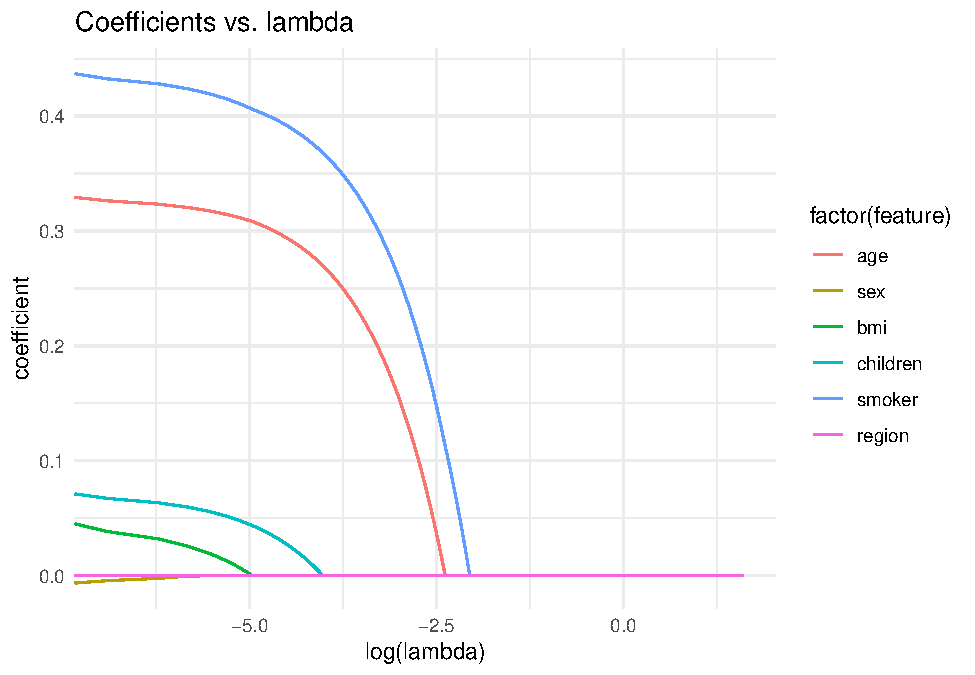
\includegraphics{assessment-1_files/figure-latex/unnamed-chunk-18-1.pdf}
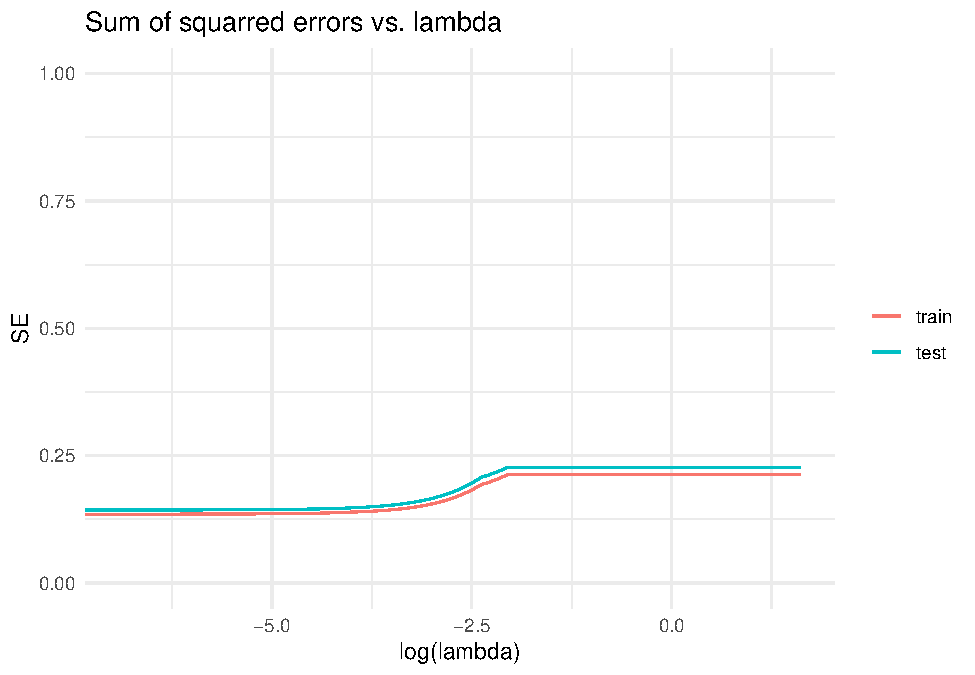
\includegraphics{assessment-1_files/figure-latex/unnamed-chunk-18-2.pdf}

\begin{Shaded}
\begin{Highlighting}[]
\CommentTok{##Ridge Regularisation }
\KeywordTok{fitAndPlot}\NormalTok{ (train.data1, train.label, }\DataTypeTok{alpha=}\DecValTok{0}\NormalTok{, }\DataTypeTok{lambda =} \KeywordTok{c}\NormalTok{(}\DecValTok{0}\OperatorTok{:}\DecValTok{5000}\NormalTok{)}\OperatorTok{/}\DecValTok{1000}\NormalTok{)}
\end{Highlighting}
\end{Shaded}

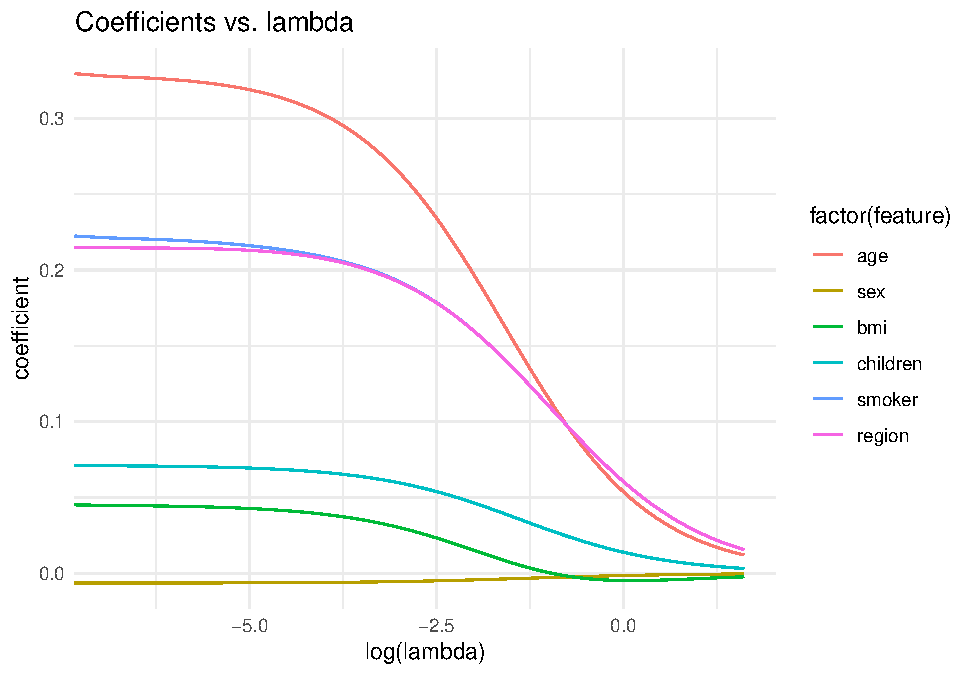
\includegraphics{assessment-1_files/figure-latex/unnamed-chunk-18-3.pdf}
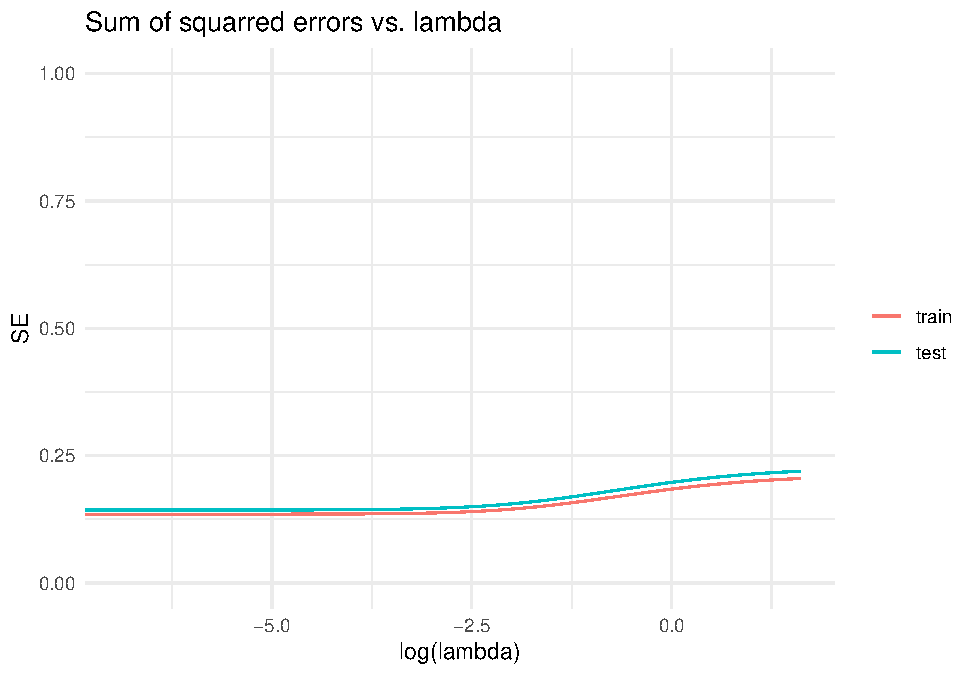
\includegraphics{assessment-1_files/figure-latex/unnamed-chunk-18-4.pdf}
\#\# Question 3 - Logistic Regression (45 marks) 1

In this question, you are required to implement a Logistic Regression
model to classify whether a person donated blood at a Blood Transfusion
Service Center in March 2007. Please read the sub-questions below
carefully for the deteailed instructions.

\begin{enumerate}
\def\labelenumi{\arabic{enumi}.}
\tightlist
\item
  Check out the Blood Transfusion Service Center Data Set at
  \url{https://archive.ics.uci.edu/ml/datasets/Blood+Transfusion+Service+Center}.
\item
  Perform data preprocessing to determine and remove invalid samples.
  Split the data into a training set and a test set with a ratio of 7:3.
  (2 marks)
\end{enumerate}

\begin{Shaded}
\begin{Highlighting}[]
\CommentTok{#read in transfusion data file }
\NormalTok{transfusion <-}\StringTok{ }\KeywordTok{read.csv}\NormalTok{(}\StringTok{'transfusion.data'}\NormalTok{)}

\CommentTok{#perform data pre-processing }
\KeywordTok{sum}\NormalTok{(}\KeywordTok{is.na}\NormalTok{(transfusion)) }\CommentTok{#appears to be no missing values }
\end{Highlighting}
\end{Shaded}

\begin{verbatim}
## [1] 0
\end{verbatim}

\begin{Shaded}
\begin{Highlighting}[]
\KeywordTok{summary}\NormalTok{(transfusion)}
\end{Highlighting}
\end{Shaded}

\begin{verbatim}
##  Recency..months. Frequency..times. Monetary..c.c..blood. Time..months.  
##  Min.   : 0.000   Min.   : 1.000    Min.   :  250         Min.   : 2.00  
##  1st Qu.: 2.750   1st Qu.: 2.000    1st Qu.:  500         1st Qu.:16.00  
##  Median : 7.000   Median : 4.000    Median : 1000         Median :28.00  
##  Mean   : 9.507   Mean   : 5.515    Mean   : 1379         Mean   :34.28  
##  3rd Qu.:14.000   3rd Qu.: 7.000    3rd Qu.: 1750         3rd Qu.:50.00  
##  Max.   :74.000   Max.   :50.000    Max.   :12500         Max.   :98.00  
##  whether.he.she.donated.blood.in.March.2007
##  Min.   :0.000                             
##  1st Qu.:0.000                             
##  Median :0.000                             
##  Mean   :0.238                             
##  3rd Qu.:0.000                             
##  Max.   :1.000
\end{verbatim}

\begin{Shaded}
\begin{Highlighting}[]
\CommentTok{##check for outliers }
\NormalTok{outliers.recency <-}\StringTok{ }\KeywordTok{boxplot.stats}\NormalTok{(transfusion}\OperatorTok{$}\NormalTok{Recency..months.)}\OperatorTok{$}\NormalTok{out}
\KeywordTok{boxplot}\NormalTok{(transfusion}\OperatorTok{$}\NormalTok{Recency..months., }\DataTypeTok{main =} \StringTok{"Recency..months."}\NormalTok{, }\DataTypeTok{boxwex =} \FloatTok{0.1}\NormalTok{)}
\KeywordTok{mtext}\NormalTok{(}\KeywordTok{paste}\NormalTok{(}\StringTok{"Outliers: "}\NormalTok{, }\KeywordTok{paste}\NormalTok{(outliers.recency, }\DataTypeTok{collapse =} \StringTok{", "}\NormalTok{)), }\DataTypeTok{cex =} \FloatTok{0.6}\NormalTok{)}
\end{Highlighting}
\end{Shaded}

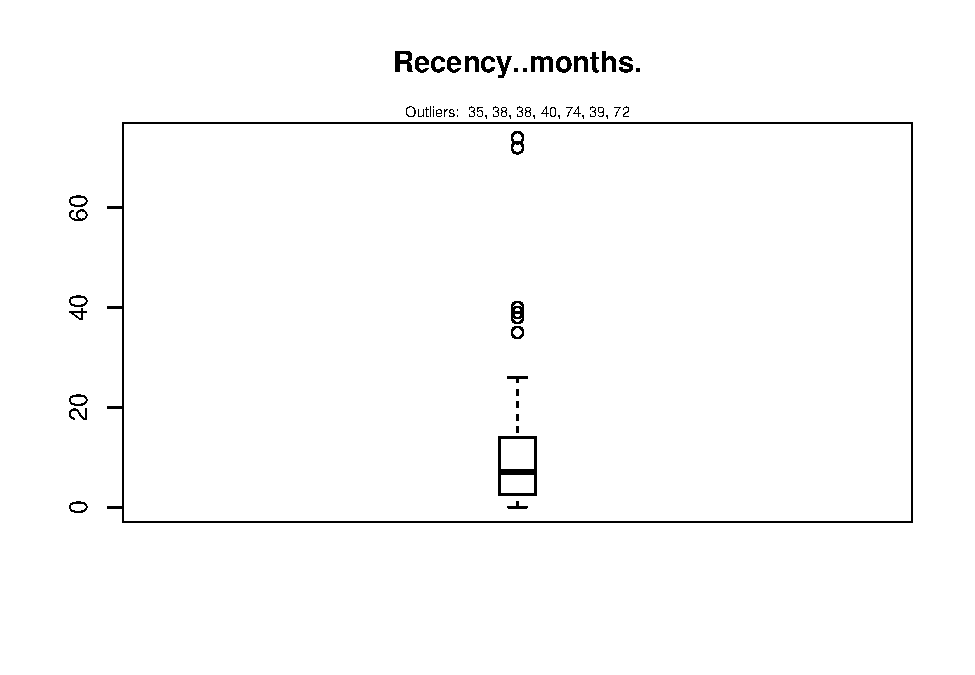
\includegraphics{assessment-1_files/figure-latex/unnamed-chunk-19-1.pdf}

\begin{Shaded}
\begin{Highlighting}[]
\NormalTok{outliers.freq <-}\StringTok{ }\KeywordTok{boxplot.stats}\NormalTok{(transfusion}\OperatorTok{$}\NormalTok{Frequency..times.)}\OperatorTok{$}\NormalTok{out}
\KeywordTok{boxplot}\NormalTok{(transfusion}\OperatorTok{$}\NormalTok{Frequency..times., }\DataTypeTok{main =} \StringTok{"Frequency..times."}\NormalTok{, }\DataTypeTok{boxwex =} \FloatTok{0.1}\NormalTok{)}
\KeywordTok{mtext}\NormalTok{(}\KeywordTok{paste}\NormalTok{(}\StringTok{"Outliers: "}\NormalTok{, }\KeywordTok{paste}\NormalTok{(outliers.freq, }\DataTypeTok{collapse =} \StringTok{", "}\NormalTok{)), }\DataTypeTok{cex =} \FloatTok{0.6}\NormalTok{)}
\end{Highlighting}
\end{Shaded}

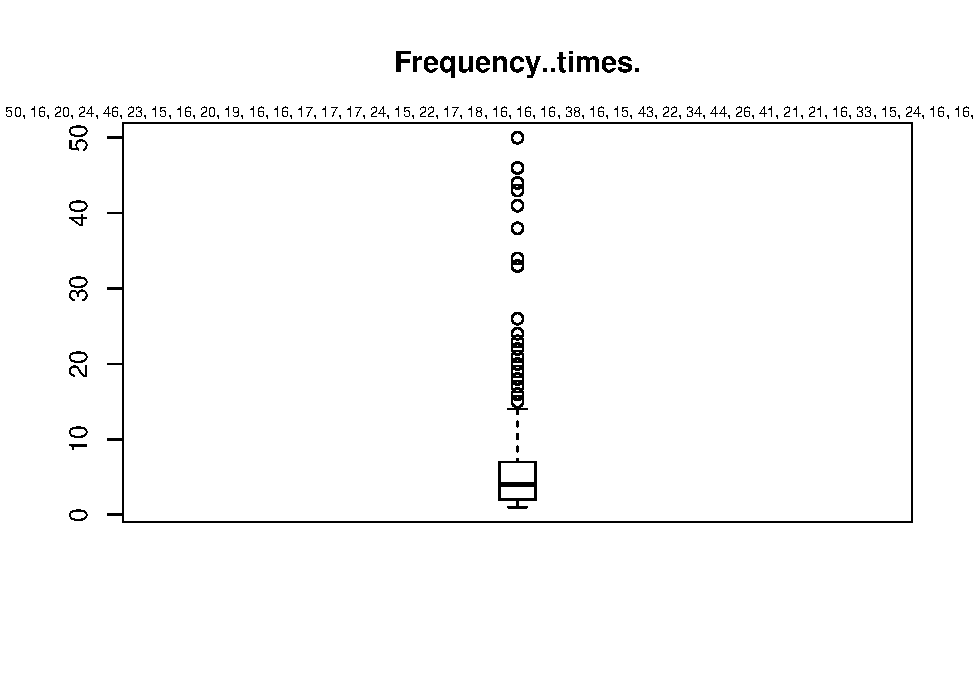
\includegraphics{assessment-1_files/figure-latex/unnamed-chunk-19-2.pdf}

\begin{Shaded}
\begin{Highlighting}[]
\NormalTok{outliers.monetary <-}\StringTok{ }\KeywordTok{boxplot.stats}\NormalTok{(transfusion}\OperatorTok{$}\NormalTok{Monetary..c.c..blood.)}\OperatorTok{$}\NormalTok{out}
\KeywordTok{boxplot}\NormalTok{(transfusion}\OperatorTok{$}\NormalTok{Monetary..c.c..blood., }\DataTypeTok{main =} \StringTok{"Monetary..c.c..blood"}\NormalTok{, }\DataTypeTok{boxwex =} \FloatTok{0.1}\NormalTok{)}
\KeywordTok{mtext}\NormalTok{(}\KeywordTok{paste}\NormalTok{(}\StringTok{"Outliers: "}\NormalTok{, }\KeywordTok{paste}\NormalTok{(outliers.monetary, }\DataTypeTok{collapse =} \StringTok{", "}\NormalTok{)), }\DataTypeTok{cex =} \FloatTok{0.6}\NormalTok{)}
\end{Highlighting}
\end{Shaded}

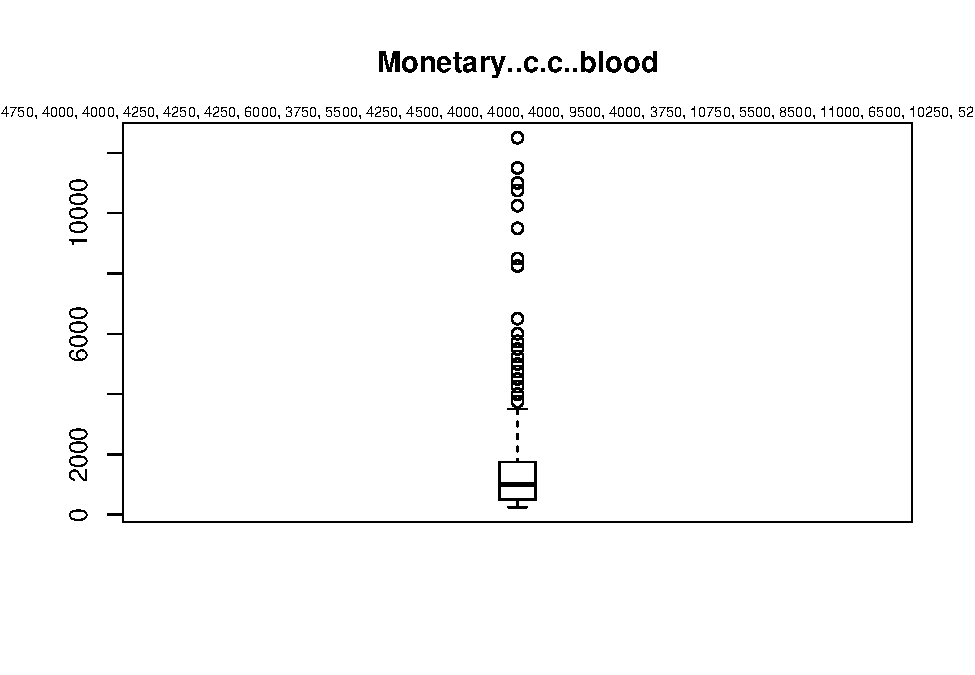
\includegraphics{assessment-1_files/figure-latex/unnamed-chunk-19-3.pdf}

\begin{Shaded}
\begin{Highlighting}[]
\NormalTok{outliers.time <-}\StringTok{ }\KeywordTok{boxplot.stats}\NormalTok{(transfusion}\OperatorTok{$}\NormalTok{Time..months.)}\OperatorTok{$}\NormalTok{out}
\KeywordTok{boxplot}\NormalTok{(transfusion}\OperatorTok{$}\NormalTok{Time..months., }\DataTypeTok{main =} \StringTok{"Time..months."}\NormalTok{, }\DataTypeTok{boxwex =} \FloatTok{0.1}\NormalTok{)}
\KeywordTok{mtext}\NormalTok{(}\KeywordTok{paste}\NormalTok{(}\StringTok{"Outliers: "}\NormalTok{, }\KeywordTok{paste}\NormalTok{(outliers.time, }\DataTypeTok{collapse =} \StringTok{", "}\NormalTok{)), }\DataTypeTok{cex =} \FloatTok{0.6}\NormalTok{)}
\end{Highlighting}
\end{Shaded}

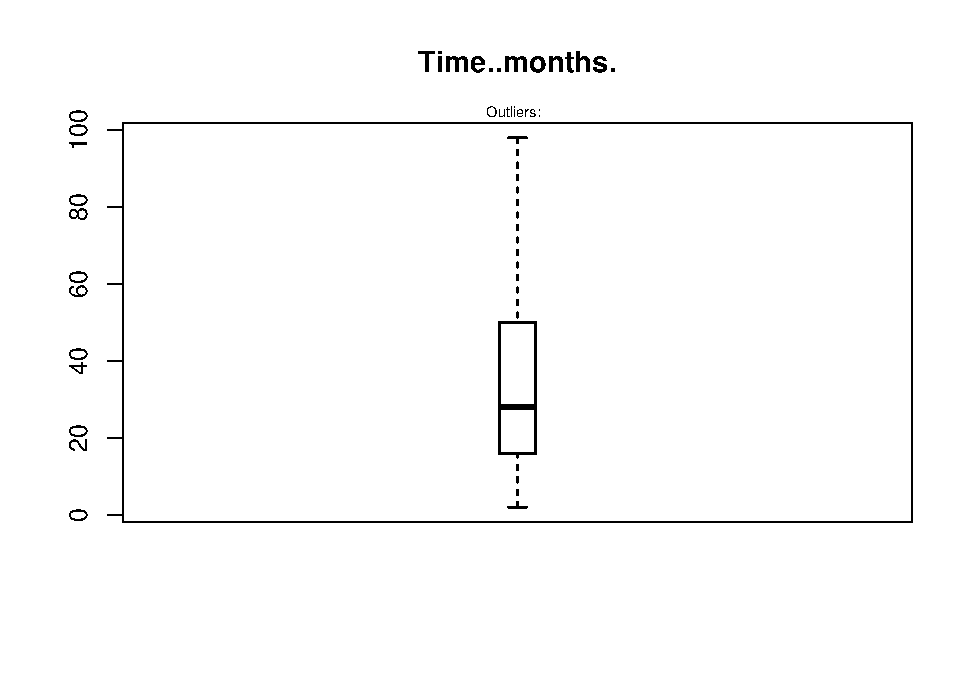
\includegraphics{assessment-1_files/figure-latex/unnamed-chunk-19-4.pdf}

\begin{Shaded}
\begin{Highlighting}[]
\CommentTok{#find which rows contain Recency outliers and remove rows}
\NormalTok{transfusion[}\KeywordTok{which}\NormalTok{(transfusion}\OperatorTok{$}\NormalTok{Recency..months. }\OperatorTok\StringTok{ }\NormalTok{outliers.recency), ]}
\end{Highlighting}
\end{Shaded}

\begin{verbatim}
##     Recency..months. Frequency..times. Monetary..c.c..blood. Time..months.
## 496               35                 3                   750            64
## 497               38                 1                   250            38
## 498               38                 1                   250            38
## 499               40                 1                   250            40
## 500               74                 1                   250            74
## 747               39                 1                   250            39
## 748               72                 1                   250            72
##     whether.he.she.donated.blood.in.March.2007
## 496                                          0
## 497                                          0
## 498                                          0
## 499                                          0
## 500                                          0
## 747                                          0
## 748                                          0
\end{verbatim}

\begin{Shaded}
\begin{Highlighting}[]
\NormalTok{transfusion <-}\StringTok{ }\NormalTok{transfusion[}\OperatorTok{-}\KeywordTok{which}\NormalTok{(transfusion}\OperatorTok{$}\NormalTok{Recency..months. }\OperatorTok\StringTok{ }\NormalTok{outliers.recency), ]}

\CommentTok{#find which rows contain Frequency outliers and remove rows}
\NormalTok{transfusion[}\KeywordTok{which}\NormalTok{(transfusion}\OperatorTok{$}\NormalTok{Frequency..times. }\OperatorTok\StringTok{ }\NormalTok{outliers.freq), ]}
\end{Highlighting}
\end{Shaded}

\begin{verbatim}
##     Recency..months. Frequency..times. Monetary..c.c..blood. Time..months.
## 1                  2                50                 12500            98
## 3                  1                16                  4000            35
## 4                  2                20                  5000            45
## 5                  1                24                  6000            77
## 10                 5                46                 11500            98
## 11                 4                23                  5750            58
## 18                 2                15                  3750            49
## 35                 2                16                  4000            64
## 45                 4                20                  5000            69
## 56                 4                19                  4750            69
## 59                 2                16                  4000            81
## 66                 3                16                  4000            74
## 73                 4                17                  4250            71
## 97                 3                17                  4250            86
## 106                6                17                  4250            70
## 116               11                24                  6000            64
## 189                8                15                  3750            77
## 242               11                22                  5500            98
## 244               11                17                  4250            79
## 279               14                18                  4500            78
## 281               14                16                  4000            70
## 321               15                16                  4000            82
## 328               14                16                  4000            98
## 342               23                38                  9500            98
## 360               21                16                  4000            64
## 367               23                15                  3750            57
## 501                2                43                 10750            86
## 502                6                22                  5500            28
## 503                2                34                  8500            77
## 504                2                44                 11000            98
## 505                0                26                  6500            76
## 506                2                41                 10250            98
## 507                3                21                  5250            42
## 509                2                21                  5250            52
## 515                4                16                  4000            38
## 518                4                33                  8250            98
## 528                2                15                  3750            64
## 529                5                24                  6000            79
## 543                4                16                  4000            70
## 563                4                16                  4000            98
## 634               12                15                  3750            71
## 636               11                16                  4000            89
## 656               16                16                  4000            77
## 673               16                15                  3750            87
## 678               23                19                  4750            62
##     whether.he.she.donated.blood.in.March.2007
## 1                                            1
## 3                                            1
## 4                                            1
## 5                                            0
## 10                                           1
## 11                                           0
## 18                                           1
## 35                                           0
## 45                                           1
## 56                                           1
## 59                                           0
## 66                                           0
## 73                                           1
## 97                                           0
## 106                                          0
## 116                                          0
## 189                                          0
## 242                                          0
## 244                                          1
## 279                                          0
## 281                                          0
## 321                                          0
## 328                                          0
## 342                                          0
## 360                                          0
## 367                                          0
## 501                                          1
## 502                                          1
## 503                                          1
## 504                                          0
## 505                                          1
## 506                                          1
## 507                                          1
## 509                                          1
## 515                                          1
## 518                                          1
## 528                                          0
## 529                                          0
## 543                                          1
## 563                                          1
## 634                                          0
## 636                                          0
## 656                                          0
## 673                                          0
## 678                                          0
\end{verbatim}

\begin{Shaded}
\begin{Highlighting}[]
\NormalTok{transfusion <-}\StringTok{ }\NormalTok{transfusion[}\OperatorTok{-}\KeywordTok{which}\NormalTok{(transfusion}\OperatorTok{$}\NormalTok{Frequency..times. }\OperatorTok\StringTok{ }\NormalTok{outliers.freq), ]}
\end{Highlighting}
\end{Shaded}

\begin{Shaded}
\begin{Highlighting}[]
\NormalTok{ nor <-}\ControlFlowTok{function}\NormalTok{(x) \{ (x }\OperatorTok{-}\KeywordTok{min}\NormalTok{(x))}\OperatorTok{/}\NormalTok{(}\KeywordTok{max}\NormalTok{(x)}\OperatorTok{-}\KeywordTok{min}\NormalTok{(x))   \}}
 
 \CommentTok{##Run nomalization on first 4 coulumns of dataset because they are the predictors}
\NormalTok{ transfusion_norm <-}\StringTok{ }\KeywordTok{as.data.frame}\NormalTok{(}\KeywordTok{lapply}\NormalTok{(transfusion, nor))}
\NormalTok{ran <-}\StringTok{ }\KeywordTok{sample}\NormalTok{(}\DecValTok{1}\OperatorTok{:}\KeywordTok{nrow}\NormalTok{(transfusion), }\FloatTok{0.7} \OperatorTok{*}\StringTok{ }\KeywordTok{nrow}\NormalTok{(transfusion)) }
\NormalTok{transfusion.x <-}\StringTok{ }\NormalTok{transfusion[ran, }\DecValTok{-5}\NormalTok{]}
\NormalTok{transfusion.y <-}\StringTok{ }\NormalTok{transfusion[ran, }\DecValTok{5}\NormalTok{]}
\end{Highlighting}
\end{Shaded}

\begin{enumerate}
\def\labelenumi{\arabic{enumi}.}
\setcounter{enumi}{2}
\tightlist
\item
  Develop a Logistic Regression model that use batch gradient descent
  for optimization. Visualize the parameter updating process, test error
  (ACC) in each iteration, and the cost convergence process. Please note
  that you need to develop your model step-by-step, built-in models in
  any realeased R package, like glm, is not allowed to use in this
  question. (10 marks)
\end{enumerate}

\begin{Shaded}
\begin{Highlighting}[]
\CommentTok{# auxiliary function that predicts class labels}
\NormalTok{predict <-}\StringTok{ }\ControlFlowTok{function}\NormalTok{(w, X, c0, c1)\{}
\NormalTok{    sig <-}\StringTok{ }\KeywordTok{sigmoid}\NormalTok{(w, X)}
    \KeywordTok{return}\NormalTok{(}\KeywordTok{ifelse}\NormalTok{(sig}\OperatorTok{>}\FloatTok{0.5}\NormalTok{, c1,c0))}
\NormalTok{\}}
    
\CommentTok{# auxiliary function that calculate a cost function}
\NormalTok{cost <-}\StringTok{ }\ControlFlowTok{function}\NormalTok{ (w, X, T, c0)\{}
\NormalTok{    sig <-}\StringTok{ }\KeywordTok{sigmoid}\NormalTok{(w, X)}
    \KeywordTok{return}\NormalTok{(}\KeywordTok{sum}\NormalTok{(}\KeywordTok{ifelse}\NormalTok{(T}\OperatorTok{==}\NormalTok{c0, }\DecValTok{1}\OperatorTok{-}\NormalTok{sig, sig)))}
\NormalTok{\}}
\end{Highlighting}
\end{Shaded}

\begin{Shaded}
\begin{Highlighting}[]
\CommentTok{# Sigmoid function (=p(C1|X))}
\NormalTok{sigmoid <-}\StringTok{ }\ControlFlowTok{function}\NormalTok{(w, x)\{}
    \KeywordTok{return}\NormalTok{(}\FloatTok{1.0}\OperatorTok{/}\NormalTok{(}\FloatTok{1.0}\OperatorTok{+}\KeywordTok{exp}\NormalTok{(}\OperatorTok{-}\NormalTok{w}\OperatorTok\KeywordTok{t}\NormalTok{(}\KeywordTok{cbind}\NormalTok{(}\DecValTok{1}\NormalTok{,x)))))    }
\NormalTok{\}}
\end{Highlighting}
\end{Shaded}

\begin{Shaded}
\begin{Highlighting}[]
\CommentTok{# Initializations}
\CommentTok{# tau.max <- 1000 # maximum number of iterations}
\CommentTok{# eta <- 0.01 # learning rate}
\CommentTok{# epsilon <- 0.01 # a threshold on the cost (to terminate the process)}
\CommentTok{# tau <- 1 # iteration counter}
\CommentTok{# terminate <- FALSE}

\CommentTok{## Just a few name/type conversion to make the rest of the code easy to follow}
\CommentTok{# X <- as.matrix(train.data) # rename just for conviniance}
\CommentTok{# T <- ifelse(train.label==c0,0,1) # rename just for conviniance}

\CommentTok{# W <- matrix(,nrow=tau.max, ncol=(ncol(X)+1)) # to be used to store the estimated coefficients}
\CommentTok{# W[1,] <- runif(ncol(W)) # initial weight (any better idea?)}

\CommentTok{# project data using the sigmoid function (just for convenient)}
\CommentTok{# Y <- sigmoid(W[1,],X)}

\CommentTok{# costs <- data.frame('tau'=1:tau.max)  # to be used to trace the cost in each iteration}
\CommentTok{# costs[1, 'cost'] <- cost(W[1,],X,T, c0)}
\end{Highlighting}
\end{Shaded}

\begin{Shaded}
\begin{Highlighting}[]
\CommentTok{# while(!terminate)\{}
    \CommentTok{# check termination criteria:}
    \CommentTok{# terminate <- tau >= tau.max | cost(W[tau,],X,T, c0)<=epsilon}
    
    \CommentTok{# shuffle data:}
    \CommentTok{# X <- X[train.index,]}
    \CommentTok{# T <- T[train.index]}
    
    \CommentTok{# for each datapoint:}
    \CommentTok{# for (i in 1:train.len)\{}
        \CommentTok{# check termination criteria:}
        \CommentTok{# if (tau >= tau.max | cost(W[tau,],X,T, c0) <=epsilon) \{terminate<-TRUE;break\}}
        
        \CommentTok{# Y <- sigmoid(W[tau,],X)}
            
        \CommentTok{# Update the weights}
        \CommentTok{# W[(tau+1),] <- W[tau,] - eta * (Y[i]-T[i]) * cbind(1, t(X[i,]))}
        
        \CommentTok{# record the cost:}
        \CommentTok{# costs[(tau+1), 'cost'] <- cost(W[tau,],X,T, c0)}
        
        \CommentTok{# update the counter:}
        \CommentTok{# tau <- tau + 1}
        
        \CommentTok{# decrease learning rate:}
        \CommentTok{# eta = eta * 0.999}
    \CommentTok{# \}}
\CommentTok{# \}}
\CommentTok{# Done!}
\CommentTok{# costs <- costs[1:tau, ] # remove the NaN tail of the vector (in case of early stopping)}

\CommentTok{# the  final result is:}
\CommentTok{# w <- W[tau,]}
\CommentTok{# cat('\textbackslash{}nThe  final coefficents are:',w)}
\end{Highlighting}
\end{Shaded}

\begin{Shaded}
\begin{Highlighting}[]
\CommentTok{#model <- logistic_regression_gradient_decent(transfusion.x, transfusion.y, )}
\end{Highlighting}
\end{Shaded}

\begin{enumerate}
\def\labelenumi{\arabic{enumi}.}
\setcounter{enumi}{3}
\tightlist
\item
  Invesitigate the influence of different learning rate to the training
  process and answer what happend if you apply a too small or a too
  large learning rate. (5 marks)
\item
  Expermently compare batch gradient descent and stochastic gradient
  descent and discuss your findings (e.g., convergence speed). Visualize
  the comparison in terms of updating process and the cost convergence
  process. (6 marks)
\item
  Develop a K-fold (K = 5) cross validation to evaluate your model in
  step 3. Please note that you need to write R codes to explicitly show
  how you perform the K-fold cross validation. Built-in validation
  methods are not allowed to use. Different metrics, e.g.~ACC, Recall,
  precision, etc, should be used to evaluate your model. (8 marks)
\item
  Use different values of K (from 5 to N, where N denotes the sample
  number) and summarize the corresponding changes of your model
  performances. Visualize and explain the changes. (6 marks)
\item
  How can you modify the cost function to prevent overfitting? Discuss
  the possibility of adding regularization term(s) and summarize the
  possible changes in the gradient descent process. (8 marks)
\end{enumerate}

\end{document}
